\documentclass[compress]{beamer}
\mode<presentation>
\setbeamercovered{transparent}
\usetheme{Warsaw}
%\useoutertheme{smoothtree}
\usepackage{multirow}
\usepackage[english]{babel}
\usepackage[latin1]{inputenc}
\usepackage{times}
\usepackage[T1]{fontenc}
\usepackage{xmpmulti}
\usepackage{multicol}
\usepackage{colortbl}
\usepackage{fixpauseincludegraphics}

%\setbeamersize{text margin left=.25 in,text margin right=.25 in}
\setbeamersize{text margin left=.15 in,text margin right=.15 in}
\usepackage[authoryear]{natbib}


\usepackage{epstopdf}
\usepackage{xcolor}
\usepackage{latexcolors}
%\usepackage[dvipsnames]{xcolor}
\definecolor{antiquebrass}{rgb}{0.8, 0.58, 0.46}
\definecolor{babyblueeyes}{rgb}{0.63, 0.79, 0.95}
\definecolor{babyblue}{rgb}{0.54, 0.81, 0.94}
\definecolor{bistre}{rgb}{0.24, 0.17, 0.12}
\definecolor{brightlavender}{rgb}{0.75, 0.58, 0.89}
\definecolor{bulgarianrose}{rgb}{0.28, 0.02, 0.03}
\definecolor{slateblue}{rgb}{0.56, 0.74, 0.56}
\definecolor{cordovan}{rgb}{0.54, 0.25, 0.27}
\definecolor{darkbyzantium}{rgb}{0.36, 0.22, 0.33}

\setbeamercolor{structure}{fg=antiquefuchsia!80, bg= black!60}







\usepackage{tikz}
\usetikzlibrary{shadows,calc}
\usetikzlibrary{shadows.blur}
\usetikzlibrary{shapes.symbols}
\usepackage{hyperref}
\usepackage{booktabs}
\usepackage{colortbl}
\usepackage{multirow}
%%%%%%%%% shaddow image %%%%%
% some parameters for customization
\def\shadowshift{3pt,-3pt}
\def\shadowradius{6pt}
\colorlet{innercolor}{black!60}
\colorlet{outercolor}{gray!05}
% this draws a shadow under a rectangle node
\newcommand\drawshadow[1]{
\begin{pgfonlayer}{shadow}
    \shade[outercolor,inner color=innercolor,outer color=outercolor] ($(#1.south west)+(\shadowshift)+(\shadowradius/2,\shadowradius/2)$) circle (\shadowradius);
    \shade[outercolor,inner color=innercolor,outer color=outercolor] ($(#1.north west)+(\shadowshift)+(\shadowradius/2,-\shadowradius/2)$) circle (\shadowradius);
    \shade[outercolor,inner color=innercolor,outer color=outercolor] ($(#1.south east)+(\shadowshift)+(-\shadowradius/2,\shadowradius/2)$) circle (\shadowradius);
    \shade[outercolor,inner color=innercolor,outer color=outercolor] ($(#1.north east)+(\shadowshift)+(-\shadowradius/2,-\shadowradius/2)$) circle (\shadowradius);
    \shade[top color=innercolor,bottom color=outercolor] ($(#1.south west)+(\shadowshift)+(\shadowradius/2,-\shadowradius/2)$) rectangle ($(#1.south east)+(\shadowshift)+(-\shadowradius/2,\shadowradius/2)$);
    \shade[left color=innercolor,right color=outercolor] ($(#1.south east)+(\shadowshift)+(-\shadowradius/2,\shadowradius/2)$) rectangle ($(#1.north east)+(\shadowshift)+(\shadowradius/2,-\shadowradius/2)$);
    \shade[bottom color=innercolor,top color=outercolor] ($(#1.north west)+(\shadowshift)+(\shadowradius/2,-\shadowradius/2)$) rectangle ($(#1.north east)+(\shadowshift)+(-\shadowradius/2,\shadowradius/2)$);
    \shade[outercolor,right color=innercolor,left color=outercolor] ($(#1.south west)+(\shadowshift)+(-\shadowradius/2,\shadowradius/2)$) rectangle ($(#1.north west)+(\shadowshift)+(\shadowradius/2,-\shadowradius/2)$);
    \shade[outercolor,right color=innercolor,left color=innercolor] ($(#1.north west)+(-\shadowradius/12,\shadowradius/12)$) rectangle ($(#1.south east)+(\shadowradius/12,-\shadowradius/12)$);%Frame
    \filldraw ($(#1.south west)+(\shadowshift)+(\shadowradius/2,\shadowradius/2)$) rectangle ($(#1.north east)+(\shadowshift)-(\shadowradius/2,\shadowradius/2)$);
\end{pgfonlayer}
}
% create a shadow layer, so that we don't need to worry about overdrawing other things
\pgfdeclarelayer{shadow} 
\pgfsetlayers{shadow,main}
% Define image shadow command
\newcommand\shadowimage[2][]{%
\begin{tikzpicture}
\node[anchor=south west,inner sep=0] (image) at (0,0) {\includegraphics[#1]{#2}};
\drawshadow{image}
\end{tikzpicture}}
\usepackage{calligra}

\DeclareMathOperator*{\argmax}{Arg\,max}
\DeclareMathOperator*{\argmin}{Arg\,min}
\newcommand{\norm}[1]{\left\Vert #1 \right\Vert }
\newcommand{\bbetaHat}{ \widehat{\bbeta}}
\newcommand{\bbetaLSE}{ \widehat{\bbeta}_{_{\text{LSE}}}}
\newcommand{\bbetaMLE}{ \widehat{\bbeta}_{_{\text{MLE}}}}
\newcommand{\sqBullet}[1]{  {\tiny \tiny \tiny \qBoxCol{#1!60}{ }} }
%***************
%\newtheorem{thm}{Theorem}
%\documentclass[noinfoline]{imsart}
%\usepackage{amsmath,amstext,amssymb}
%%\usepackage[top=1.5in, bottom=1.5in, left=1.2in, right=1.2in]{geometry}
%% settings
%%\pubyear{2005}
%%\volume{0}
%%\issue{0}
%%\firstpage{1}
%%\lastpage{8}
%\arxiv{arXiv:0000.0000}

%\startlocaldefs
%\numberwithin{equation}{section}
%\theoremstyle{plain}
%\newtheorem{thm}{Theorem}
%\endlocaldefs
\usepackage{lipsum} 
\usepackage{amsmath}
\usepackage{amssymb}
\usepackage{amsbsy} 
\usepackage{amsthm}
\usepackage{mathrsfs}
\usepackage{eufrak}
\usepackage{mathrsfs}
\usepackage{color}
\usepackage{verbatim}
\usepackage{graphicx}
\usepackage{bm}
\usepackage{enumerate}
\usepackage{epstopdf} 
\usepackage{natbib}
\usepackage{undertilde}
%\RequirePackage[colorlinks,citecolor=blue,urlcolor=blue]{hyperref}
%\usepackage{subfig}
\usepackage[final]{pdfpages}

\usepackage{algorithm}  %@subhajit
\usepackage{algpseudocode} %@subhajit
\usepackage{algorithmicx}     %@subhajit
\usepackage{undertilde}


\newcommand{\sphere}{{\mathbb{S}}}
\newcommand{\R}{\mathbb{R}}
\newcommand{\LatentV}{V}
\newcommand{\NC}{m}
\newcommand{\Priorf}{f_{prior}}
\newcommand{\FWOne}[2]{{{}_{1}\Psi _{1}\left[{\begin{matrix}(\frac{#1}{2},\frac{1}{2})\\(1,0)\end{matrix}};#2\right]} 
}


\newcommand{\HyPriorMu}{\thetabf}
\newcommand{\HyPriorAlpha}{\alpha}
\newcommand{\HyPriorBeta}{\beta}
\newcommand{\HyPriorK}{\zeta}
\newcommand{\Indicator}[2]{\mathbb{I}_{_{#1}}({#2 })}
\newcommand{\xb}{\bm{x}}
\newcommand{\bx}{\MakeVec{\bm{x}}}
\newcommand{\bX}{\bm{X}}
\newcommand{\by}{\MakeVec{\bm{y}}}
\newcommand{\bZ}{\bm{Z}}
\newcommand{\bF}{\bm{F}}
\newcommand{\btheta}{\MakeVec{{\bm{\theta}}}}
\newcommand{\Bpi}{\MakeVec{\boldsymbol{\pi}}}
\newcommand{\thetabf}{\MakeVec{\boldsymbol{\theta}}}
\newcommand{\Thetabf}{\boldsymbol{\Theta}}
\newcommand{\taubf}{\MakeVec{\boldsymbol{\tau}}}
\newcommand{\Tr}{Tr}


\newcommand{\bM}{\bm{M}}
\newcommand{\bD}{\MakeVec{\bm{D}}}
\newcommand{\bV}{\MakeVec{\bm{V}}}
\newcommand{\loglikmix}{\mathcal{L}_{\bM,\bD,\bV}}
\newcommand{\hypdc}{{}_0F_1\left(\frac{n}{2},\frac{D_c^2}{4}\right)}


\usepackage{xstring}
\usepackage[normalem]{ulem}
\definecolor{ultramarine}{RGB}{38,29,163}
\newcommand\PalDel[1]{{\color{red} {\sout{#1}}}}
\newcommand\Pal[1]{{\color{ultramarine}{#1}}}
\newcommand\PalRp[2]{\PalDel{#1} \Pal{#2}}
\newcommand\PalCmnt[1]{{\color{ultramarine} {[[[***PAL:  #1 ***]]]}}}

\newcommand{\qedwhite}{\hfill \ensuremath{\Box}}
\newcommand{\SpaceD}{\mathcal{S}_p}
\newcommand{\SpaceM}{\widetilde{\mathcal{V}}_{n,p}}
\newcommand{\SpaceV}{\mathcal{V}_{p,p}}
\newcommand{\SpaceF}{\mathbb{R}^{n,p}}
\newcommand{\StiefelS}{\mathcal{V}_{n,p}}
\newcommand{\SpacePi}{\mathbb{S}_{\pi}}
\newcommand{\ML}{{\cal{ML}}}
\newcommand{\ProdSpace}{\boldsymbol{\Theta}}
\newcommand{\ThetaAndPi}{\Xi}
\newcommand{\ClassML}{\mathcal{C}_{\ML}}


\newcommand{\balpha}{\MakeVec{\bm{\alpha}}}
\newcommand{\bbeta}{\MakeVec{\bm{\beta}}}
\newcommand{\bEta}{\bm{\eta}}
\newcommand{\bd}{{\utilde{\bm{d}}}}
\newcommand{\BoEta}{{\utilde{\boldsymbol{\eta}}}}
%\newtheorem{theorem}{Theorem}[section]
%\newtheorem{theorem}{Theorem}
%\newtheorem{lemma}{Lemma}
%\newtheorem{result}{Result}
\newtheorem{defn}{Definition}
\newcommand{\pdv}[2][]{\frac{\partial#1}{\partial#2}}
\newcommand{\pdvtwo}[2][]{\frac{\partial^2#1}{{\partial#2}^2}}


%\newcommand{\mubf}{\boldsymbol{\mu}}
\newcommand{\mubf}{\MakeVec{\mu}}
\newcommand{\sumI}{ \sum_{i=1}^{n}}
\newcommand{\Ybar}{{\overline{Y}}}

\newcommand{\Expectation}[1]{\mathbb{E}{[#1]}}
\newcommand{\priorXzero}{\Psi}
\newcommand{\iMat}{\mathbf{I}_{p}}

% 
% \newtheorem{thm}{Theorem}[section]
% \newtheorem{cor}[thm]{Corollary}
% \newtheorem{lem}[thm]{Lemma}
%\newtheorem{proposition}{Proposition}

%\newtheorem{theorem}{Theorem}[chapter]%To link the theorem to each chapter uncomment the chapter option
%\newtheorem{lemma}{Lemma}%[theorem]% To link each lemma to a theorem uncomment the theorem option
%\newtheorem{corollary}{Corollary}%[theorem]% To link each corollary to a theorem uncomment the theorem option
% to link a corollary to a chapter change the theorem option to chapter
%\newtheorem{definition}{Definition}%[chapter] %the same is true for both definitions and assumptions
\newtheorem{assumption}{Assumption}%[chapter] %
%\newtheorem{proposition}{Proposition}[chapter]
%\newtheorem{fact}{Fact} %%% added by @subho
\newcommand{\StrongNBD}[2]{S_{#1}{#2}}
\newcommand{\bpi} {\boldsymbol{\pi}}
\newcommand{\bphi} {\boldsymbol{\phi}}
\newcommand{\bb}[1]{\boldsymbol{#1}}
% Definitions of handy macros can go here

\newcommand{\normtwo}[1]{{\left\lVert#1\right\rVert}_2}

\newcommand{\dataset}{{\cal D}}
\newcommand{\fracpartial}[2]{\frac{\partial #1}{\partial  #2}}
\newcommand{\Lesbegue}[1]{\mu_{\btheta_{#1},\bpi_{#1}}}
\newcommand{\fthetapi}[1]{f_{\btheta_{#1},\bpi_{#1}}}
% Heading arguments are {volume}{year}{pages}{submitted}{published}{author-full-names}
\newcommand{\doublehat}[1]{%
    \settoheight{\dhatheight}{\ensuremath{\widehat{#1}}}%
    \addtolength{\dhatheight}{-0.35ex}%
    \widehat{\vphantom{\rule{2pt}{\dhatheight}}%
    \smash{\hspace{-0.5mm}\widehat{#1}}}}

\newcommand{\hyp}{{}_0F_1\left(\frac{n}{2},\frac{D^2}{4}\right)}
\newcommand{\hypinline}{{}_0F_1\left({n}/{2},{D^2}/{4}\right)}

\newcommand{\partialhyp}[1]{\frac{\partial}{\partial\,{d_{#1}}}\,\left[\hyp\right]}

\newcommand{\fracProbZ}[1]{\frac{\langle Z_{ic} \rangle \, #1}{\sum_{i=1}^{N} \langle Z_{ic}\rangle  } }
\newcommand{\EmVar}[1]{\widetilde{#1}^{(c)}}

\newcommand{\IMDY}{{\it{CCPD}}}
\newcommand{\JMDY}{{\it{JCPD}}}

\newcommand{\DYlang}{\frac{\exp(\nu\,\bEta^T\bd)}{{\left[{}_0F_1\left(\frac{n}{2},\frac{D^2}{4}\right)\right]}^{\nu}}}

\newcommand{\logDYlang}{\nu\,\bEta^T\bd - \nu\,\log\left({}_0F_1\left(\frac{n}{2},\frac{D^2}{4}\right)\right)}

\newcommand{\lhyp}{\log\left({}_0F_1\left(\frac{n}{2},\frac{D^2}{4}\right)\right)}

%\jmlrheading{1}{2000}{1-48}{4/00}{10/00}{SS \& JH \& AB}

% Short headings should be running head and authors last names

%\ShortHeadings{BDP and cIBP}{SS \& JH \& AB}
%\firstpageno{1}

\newcommand{\diam}[1]{{{#1}^{\ast}}}

%%% coloring option %%%
\definecolor{auburn}{rgb}{0.53, 0.1, 0.5}
\newcommand{\sss}{\color{auburn}}  %%% for Subhajit
\newcommand{\sse}{\color{black}}
\newcommand{\attn}{\color{red}}
\newcommand{\rms}{\color{magenta}}  %%% for Riten
\newcommand{\rme}{\color{black}}
\newcommand{\MLDensity}{f_{\ML}}
\setlength{\parindent}{0cm}
\newcommand{\posterior}

\newcommand{\variableX}{\bd}
\newcommand{\funch}{\mathfrak{h}}
\newcommand{\IndVzero}[1]{\mathbb{I}({X\in \mathcal{V}^{#1}_0})}
\newcommand{\Rnp}{\mathbb{R}^{n \times p}}
\newcommand{\Rpp}{\mathbb{R}^{p \times p}}
\newcommand{\vecnorm}[1]{\lVert #1\rVert}

\newcommand{\etapsiD}{\eta_{\priorXzero}}
\newcommand{\BoEtapsiD}{\BoEta_{\priorXzero}}

\newcommand{\DMp}{\mathcal{D}^{p \times p}}
\newcommand{\Rplus}{\mathbb{R}_{+}}
\newcommand{\prodMeasure}{\Upsilon}

\newcommand{\m}{{\bf m_{\BoEta}}} 
\newcommand{\SetWithMode}{\mathcal{S}}
\newcommand{\SetWithModePrime}{\mathcal{S}}
\newcommand{\TargetComp}{\mathcal{S}^{\star}}

\newcommand{\ConstCondDen}{K_{\nu, \BoEta}} 

\newcommand{\hyparam}[2]{
    \IfEqCase{#1}{
        {M}{\xi^{#2}_c}
        {V}{\gamma^{#2}_c}%
        
    }
  }
\newcommand{\threepartdef}[6]
{
	\left\{
		\begin{array}{lll}
			#1 & \mbox{if } #2 \\
			#3 & \mbox{if } #4 \\
			#5 & \mbox{if } #6
		\end{array}
	\right.
}

\def\bv{\color{blue}}
\def\ev{\color{black}}
\newcommand{\bch}{\bv }
\newcommand{\ech}{\ev\normalsize}
%\newcommand{\MakeVec}[1]{{\utilde{\bf #1}}}
\newcommand \Measure[2][]{%
  \ifstrempty{#1}{
  \IfEqCase{#2}{
        {M}{\mu}%
        {D}{\mu_1}%
        {V}{\mu_2}
        {X}{\mu}
   }  
  }{
  \IfEqCase{#1}{
  {1}{
   \IfEqCase{#2}{
        {M}{d\mu(M)}%
        {D}{d\mu_1(\bd)}%
        {V}{d\mu_2(V)}
        {X}{d\mu(X)}
        {Y}{d\mu(Y)}
        {MDV} {d\mu(M)\; d\mu_1(\bd) \;d\mu_2(V) }
        }
   } 
   {2}{
   \IfEqCase{#2}{
         {M}{d\mu(M^{\ast})}%
        {D}{d\mu_1(\bd^{\ast})}%
        {V}{d\mu_2(V^{\ast})}
        {X}{d\mu(X^{\ast})}
        }
   }
   {3}{
   \IfEqCase{#2}{
         {M}{\mu(dM^{\star})}%
        {D}{\mu_2(d\bd^{\star})}%
        {V}{\mu_1(dV^{\star})}
        {X}{\mu(X^{\star})}
        }
   }   
   
   } 
  }%
}
  \newcommand{\VONF}{\text{VonMisesFisher}}
\newcommand{\MPGalpha}{\alpha}
\newcommand{\MPGnu}{\nu}
\newcommand{\MPG}{MPG }
\newcommand{\ybin}{y^{(\text{bin})}}


%\newcommand{\abs}[1]{\left \vert  #1  \right\vert  }
\usepackage{caption}
\usepackage{subcaption}

%%%%%%%%%%%%%%%%%%%%%%%%%%%
\newcommand{\IEHC}{\text{IEHC}}







\newcommand \Th[1]{%
  \IfEqCase{#1}{
        {1}{ 1^{\text{st}}}%
        {2}{2^{\text{nd}}}%
        {3}{3^{\text{rd}}}%
  }[{#1}^{\text{th}}]
}
  
  
   \newcommand{\augV}{\text{aux}}
  
  
  
  
  \newcommand{\CDE}{\text{PL}}
\newcommand{\CDEsigma}{\sigma}
\newcommand{\CDEepsilon}{\SVepsilon}
\newcommand{\CDEmu}{\mu}
 % \newcommand{\SVepsilon}{\varepsilon}
  \newcommand{\SVepsilon}{\delta}
 \newcommand{\abs}[1]{\left\lvert{#1}\right \rvert }
 
 
\newcommand{\CPDX }{\text{CPDX}}
\newcommand{\CPDXPar}{\vartheta}
\newcommand{\K}{\mathcal{K}}



\newcommand{\lossFunctionOne}[1]{ \left\{ \abs{ ( \abs{#1}-\SVepsilon)}  + ( \abs{#1}-\SVepsilon)\right\} }

\newcommand{\lossFunctionAlt}[1]{ \abs{  #1-\SVepsilon}  + \abs{ #1+\SVepsilon}-2\SVepsilon }

\newcommand{\lossFunctionAltOne}[1]{   \lossFunctionAlt{ \frac{\left(#1\right)}{\sigma}}}

\newcommand{\lossFunction}[1]{ \left\{ \abs{ \left( \frac{\abs{#1}}{\sigma}-\SVepsilon\right)}  + \left( \frac{\abs{#1}}{\sigma}-\SVepsilon\right)\right\} }
\newcommand{  \Likelihood}{\mathcal{L}}
%\newcommand{\Onebf}{\bf 1}
\newcommand{\Onebf}{{\bf \utilde{1}_{n}}}





\newcommand{\InvGamma}{\text{InvGamma}}
\newcommand{\PriorSigmaAlpha}{a}
\newcommand{\PriorSigmaBeta}{b}
\newcommand{\PriorBetaMean}{\mubf_{_{\bbeta}}}
\newcommand{\PriorBetaVar}{\Sigma_{_{\bbeta}}  }
\newcommand{\mvnormPdf}[4]{\frac{1}{ \left({2\pi}\right)^{\frac{#4}{2}} \sqrt{\vert{#3}\vert}}{\exp\left[ - \frac{1}{2}(#1- #2)^T {#3}^{-1} (#1- #2)\right]}      }
\newcommand{\InvGammaPdf}[3]{ \frac{(#1)^{-#2+1}}{\Gamma\left( #2\right) } \exp\left[ -\frac{{#3}}{{#1}} \right] }

 \newcommand{\byTilde}{\tilde{\by}}
 
 \newcommand{\TrfSigma}{\varsigma}
 \newcommand{ \Normal}{\text{Normal}}
 \newcommand{\GlobalPar}{\tau}
\newcommand{\LocalPar}{\psi}
\newcommand{\Not}[1]{{\overline{#1}}}
\newcommand{\st}{:}

\newcommand{\define}[2]{ \begin{definition}[#1]  #2  \end{definition}  }

\newcommand{\Exmpl}[2]{\qBrd[0.75in]{#1}{Example #2:}}
\newcommand{\Qn}{\HLTW{Question:} }


\newcommand{\pmf}{p}
\newcommand{\cdf}{F}
%\NewDocumentCommand{\support}{O{ }}{{\mathcal{S}}_{_{#1}}}
\NewDocumentCommand{\support}{O{ }}{{\mathbb{S}}_{_{#1}}}
%\newcommand{\SampleS}{\mathcal{S}}
\newcommand{\SampleS}{\mathscr{S}}
\usepackage{xcolor}
\usepackage{xparse}
\definecolor{lightGray}{gray}{0.95}
\definecolor{lightGrayOne}{gray}{0.9}
\definecolor{lightBlueOne}{RGB}{204, 255, 255}
\definecolor{lightBlueTwo}{RGB}{204, 238, 255}
\definecolor{lightBlueThree}{RGB}{204, 204, 255}
\definecolor{AltBlue}{RGB}{119,14,161}
\definecolor{Orchid}{RGB}{186,85,211}

\definecolor{BGBlue}{RGB}{220,221,252}
\definecolor{BGBlueOne}{RGB}{204,229,255}

\definecolor{DarkGreenOne}{RGB}{34,139,34}

\definecolor{BGGreen}{RGB}{240,243,245}
\definecolor{lightGreenOne}{RGB}{179, 255, 179}
\definecolor{lightGreenTwo}{RGB}{198, 255, 179}
\definecolor{lightGreenThree}{RGB}{243, 255, 230}
\definecolor{AltGreen}{RGB}{193, 240, 240}

\definecolor{BOGreen}{RGB}{180,0,0}
\definecolor{BGGreenOne}{RGB}{220,250,220}

\definecolor{lightBrownOne}{RGB}{255, 221, 204}
\definecolor{lightBrownTwo}{RGB}{255, 229, 204}
\definecolor{lightBrownThree}{RGB}{242, 217, 230}


\definecolor{HLTGreen}{RGB}{230,244,215}
\definecolor{ExcBrown}{RGB}{153,0,0}
\definecolor{ExcBGBrown}{RGB}{255,204,204}
\definecolor{BGYellowOne}{RGB}{255,235,208}
\definecolor{BGPink}{RGB}{255,215,240}

\newcommand{\MakeVec}[1]{{\utilde{\bf #1}}}

\NewDocumentCommand{\MCOption}{O{1.75in} m}{
\TextInBoxTwo[BGPink]{ #1 } {\TextInBoxTwo[white]{.1 in }{ \quad}\HLT{#2}}
}

 \NewDocumentCommand{\ThreeChoices}{O{Do not Know}O{Not confident}O{Confident}}{
\MCOption{#1} \MCOption{#2} \MCOption{#3}
}
 
\NewDocumentCommand{\OneBlock}{ O{HLTGreen} m m }{\colorbox{#1}{\begin{minipage}{#2} $ #3$ \end{minipage}}}

\NewDocumentCommand{\HLT}{ O{HLTGreen} m }{\colorbox{#1}{#2}}
%\NewDocumentCommand{\HLTEQ}{ O{HLTGreen} m }{\colorbox{#1}{$#2$}}
\NewDocumentCommand{\HLTEQ}{ O{white} m }{\colorbox{#1}{$#2$}}

%\newcommand{\HLT}[1]{\colorbox{HLTGreen}{#1}}
\newcommand{\DEHLT}[1]{\colorbox{lightGrayOne}{\color{white} #1}}

\newcommand{\TextInBoxOne}[2]{  {\fcolorbox{white}{lightGrayOne}{\begin{minipage}{#1}  #2 \end{minipage}}}}


\NewDocumentCommand{\TextInBoxTwo}{ O{lightGrayOne} m m } {{\fcolorbox{white}{#1}{\begin{minipage}{#2} { #3} \end{minipage}}}}


\newcommand{\TextInBox}[2]{  {\fcolorbox{BGGreen}{BGGreen}{\begin{minipage}{#1}  #2 \end{minipage}}}}
\newcommand{\TextInBoxCol}[2]{
\fcolorbox{BGBlue}{BGBlue}{%
\begin{minipage}{#1}
 {\color{AltBlue} #2}
\end{minipage}}%
}

\NewDocumentCommand{\TxtBnd}{ O{lightBrownOne} m m } {{\fcolorbox{white}{#1}{\begin{minipage}{#2} { #3} \end{minipage}}}}


\newcommand{\BandInTopBox}[2]{
\fcolorbox{AltBlue}{AltBlue}{%
\begin{minipage}{#1}{ {\color{white}  #2 \hspace{.1in}} }
\end{minipage}}%
}


\newcommand{\TextInBoxThm}[2]{
\fcolorbox{AltBlue}{lightGray}{%
\begin{minipage}{#1}
 {\color{black} #2}
\end{minipage}}%
}

\newcommand{\TextInBoxThmOne}[2]{
\fcolorbox{BGBlue}{BGBlueOne}{%
\begin{minipage}{#1}
 {\color{AltBlue} #2}
\end{minipage}}%
}

\newcommand{\TextInBoxLem}[2]{
\fcolorbox{BGBlue}{lightGray}{%
\begin{minipage}{#1}
 {\color{black} #2}
\end{minipage}}%
}



\newcommand{\TextInBoxLemOne}[2]{
\vspace{.02 in}
\noindent
\fcolorbox{BGBlue}{BGBlue}{%
\begin{minipage}{#1}
 {\color{AltBlue} #2}
\end{minipage}}%
}



\newcommand{\DefBox}[1]{
%\vspace{.1 in}
\noindent
\TextInBoxLem{4.5 in }{
\BandInTopBox{4.4 in }{}
\TextInBoxLemOne{4.4 in }{
#1
}}}





\newcommand{\DefBoxOne}[2]{
%\vspace{.1 in}
\noindent
\TextInBoxLem{4.5 in }{
\BandInTopBox{4.4 in }{#1}
\TextInBoxLemOne{4.4 in }{
#2
}}}


\newcommand{\ThmBox}[2]{
\noindent
\TextInBoxThm{4.4 in }{
\TextInBoxThmOne{4.4 in }{
#1}
#2}
}

\newcommand{\LemBox}[2]{
\noindent
\TextInBoxLem{4.5 in }{
\TextInBoxLemOne{4.4 in }{
#1}
#2}
}

\newcommand{\PropBox}[2]{
\vspace{.1 in}
\noindent
\TextInBoxLem{4.5 in }{
\TextInBoxLemOne{4.4 in }{
#1}
#2}
}




\newcommand{\TextInBoxExc}[2]{
\noindent
\fcolorbox{white}{BGGreenOne}{%
\begin{minipage}{#1}
 {\color{black} #2}
\end{minipage}}%
}


\newcommand{\TextInBoxExample}[2]{
\noindent
\fcolorbox{white}{BGPink}{%
\begin{minipage}{#1}
 {\color{black} #2}
\end{minipage}}%
}


\newcommand{\ExerciseBox}[1]{
\noindent
%\TextInBoxLem{6 in }{
\TextInBoxExc{6 in }{
#1}
%#2}
}


\newcommand{\ExampleBox}[1]{
\noindent
%\TextInBoxLem{6 in }{
\TextInBoxExample{6 in }{
#1}
%#2}
}

\NewDocumentCommand{\CommentBox}{ O{BGBlue}  m }{
\TextInBoxLem{5.5in }{
{\bf Comment:}\\
\TextInBoxLemOne{5.4 in }{
#2}}
}



\newcommand{\HLTY}[1]{\HLTEQ[yellow]{#1}}
\newcommand{\HLTW}[1]{\HLTEQ[white]{#1}}



\newcommand{\qBox}[1]{
  \begin{tikzpicture}
\node[draw=none,shade,
      top color=lightGrayOne,
      bottom color=lightGray,
      rounded corners=2pt,
      blur shadow={shadow blur steps=5}
    ] at (0,0) {    \noindent 
\fcolorbox{white}{BGBlue}{%
\begin{minipage}{4.55 in}
 {\color{black} {
 #1}}
\end{minipage}  }%
 };
 
    \end{tikzpicture}
}
 
 


 

\newcommand{\qBoxCol}[2]{
  \begin{tikzpicture}
\node[draw=none,shade,
      top color=lightGrayOne,
      bottom color=lightGray,
      rounded corners=2pt,
      blur shadow={shadow blur steps=5}
    ] at (0,0) {    \noindent
\fcolorbox{white}{#1}{%
%\begin{minipage}{4.55 in}
\begin{minipage}{4.55 in}
 {
 \color{black} {
 #2}}
\end{minipage}  }%
 };
 
    \end{tikzpicture}
}
  
  
  
  
  
  

\NewDocumentCommand{\qBrd}{O{4.55 in} m m}{
  \begin{tikzpicture}
\node[draw=none,shade,
      top color=#2,
      bottom color=#2,
      rounded corners=2pt,
      blur shadow={shadow blur steps=5}
    ] at (0,0) {    \begin{minipage}{#1}
 {
 \color{black} {
 #3}}
\end{minipage} 

 };
 
    \end{tikzpicture}
}
    
  
  
  
  
\NewDocumentCommand{\qbx}{O{4.55 in} m m}{
  \begin{tikzpicture}
\node[draw=none,shade,
      top color=lightGrayOne,
      bottom color=lightGray,
      rounded corners=2pt,
      blur shadow={shadow blur steps=5}
    ] at (0,0) {    \noindent
\fcolorbox{white}{#2}{%
%\begin{minipage}{4.55 in}
\begin{minipage}{#1}
 {
 \color{black} {
 #3}}
\end{minipage}  }%
 };
 
    \end{tikzpicture}
}
  
 
 
 \newcommand{\CurlyBox}[1]{
\begin{center}
  \begin{tikzpicture}
    \node[tape,draw=none,shade,
      top color=blue!40,
      bottom color=blue!5,
      rounded corners=1pt,
      blur shadow={shadow blur steps=5,shadow blur extra rounding=1.3pt}
    ] at (2,0){\sffamily\bfseries\large #1};
  \end{tikzpicture}
\end{center} 
 }


\newcommand{\CmntBnd}{\BandInTopBox{4.5in}{Comment:}}
\NewDocumentCommand{\TopBand}{O{Comment:} m}{ \BandInTopBox{4.5in}{#2}}

\newcommand{\DBX}[1]{
 	\HLTEQ[AltBlue]{
 				\HLTEQ[BGBlue]{  #1  }
 	}
 }



\NewDocumentCommand{\TransitionFrame}{O{slateblue}m}{
\begin{frame}{ }
\qBoxCol{#1!40}{\vspace{.8in}  \begin{center}\qBrd[2in]{#1!70}{ \begin{center} \vspace{.1in}
  #2 \\
 \vspace{.1in}
\end{center}}\end{center}
\vspace{.7in}
}

\end{frame}

}


\newcommand \rbind[1]{%
    \saveexpandmode\expandarg
    \StrSubstitute{\noexpand#1}{,}{&}[\fooo]%
    %\StrSubstitute{\fooo}{,}{&}[\fooo]%
    \StrSubstitute{\fooo}{;}{\noexpand\\}[\fooo]%
    \StrSubstitute{\fooo}{:}{\noexpand\\}[\fooo]%
    \restoreexpandmode
   \left[ \begin{matrix}\fooo\end{matrix}\right]
    }
    
    
    
   \newcommand \ColVec[1]{%
    \saveexpandmode\expandarg
    \StrSubstitute{\noexpand#1}{,}{\noexpand\\}[\fooo]%
    %\StrSubstitute{\fooo}{,}{&}[\fooo]%
    \StrSubstitute{\fooo}{;}{\noexpand\\}[\fooo]%
    \StrSubstitute{\fooo}{:}{\noexpand\\}[\fooo]%
    \restoreexpandmode
   \left[ \begin{matrix}\fooo\end{matrix}\right]
    }
     \newcommand \RowVec[1]{%
    \saveexpandmode\expandarg
    \StrSubstitute{\noexpand#1}{,}{&}[\fooo]%
    %\StrSubstitute{\fooo}{,}{&}[\fooo]%
    \StrSubstitute{\fooo}{;}{&}[\fooo]%
    \StrSubstitute{\fooo}{:}{&}[\fooo]%
    \restoreexpandmode
   \left[ \begin{matrix}\fooo\end{matrix}\right]
    }



  \newcommand \Row[1]{%
    \saveexpandmode\expandarg
    \StrSubstitute{\noexpand#1}{,}{&}[\fooo]%
    %\StrSubstitute{\fooo}{,}{&}[\fooo]%
    \StrSubstitute{\fooo}{;}{&}[\fooo]%
    \StrSubstitute{\fooo}{:}{&}[\fooo]%
    \restoreexpandmode
    \begin{matrix}\fooo\end{matrix}
    }
        
    
    
    
    \newcommand \Col[1]{%
    \saveexpandmode\expandarg
    \StrSubstitute{\noexpand#1}{,}{\noexpand\\}[\fooo]%
    %\StrSubstitute{\fooo}{,}{&}[\fooo]%
    \StrSubstitute{\fooo}{;}{\noexpand\\}[\fooo]%
    \StrSubstitute{\fooo}{:}{\noexpand\\}[\fooo]%
    \restoreexpandmode
    \begin{matrix}\fooo\end{matrix}
    }

%%%%%%%%%%%%%%%%%%%%% Experimental %%%%%%%%%%%%%%%%%


\ExplSyntaxOn
\DeclareExpandableDocumentCommand{\replicate}{O{}mm}
 {
  \int_compare:nT { #2 > 0 }
   {
    {#3}\prg_replicate:nn {#2 - 1} { #1#3 }
   }
 }
\ExplSyntaxOff


\ExplSyntaxOn
\DeclareExpandableDocumentCommand{\repdiag}{O{}mm}
 {
  \int_compare:nT { #2 > 0 }
   {
    {\prg_replicate:nn {#2}{#3#1}}{#3}
   }
 }
\ExplSyntaxOff


\newcommand \StrRowDiag[1]{%
    \saveexpandmode\expandarg
    \StrSubstitute{\noexpand#1}{,}{&}[\fooo]%
    %\StrSubstitute{\fooo}{,}{&}[\fooo]%
    \StrSubstitute{\fooo}{;}{&}[\fooo]%
    \StrSubstitute{\fooo}{:}{&}[\fooo]%
    \StrCount{\fooo}{&}[\countfooo]
    \restoreexpandmode
    \repdiag[0]{\countfooo+1}{{,}}
   %\left[ \begin{matrix}\fooo\end{matrix}\right]
    }


\newcommand \DiagStrOne[2]{%
    \saveexpandmode\expandarg
    \StrSubstitute{\noexpand#1}{,}{\noexpand#2}[\fooo]%
    \restoreexpandmode
   %\left[ \begin{matrix}\fooo\end{matrix}\right]
   \fooo
    }
    
    \newcommand \DiagStr[1]{%
    \DiagStrOne{#1}{{\StrRowDiag{#1}}}
    }


%$\rbind{\replicate[,]{10}{\Col{\replicate[;]{7}{0}}}}$

%$\Col{1,2,3}$
%$\ColVec{\replicate[;]{5}{B}}$
%$ \StrRowDiag{1,2} $

%$\DiagStr{1,2,3}$

%\repdiag[-]{3}{A}
\ExplSyntaxOn
\NewDocumentCommand{\Split}{ m m o }
 {
  \tarass_split:nn { #1 } { #2 }
  \IfNoValueTF { #3 } { \tl_use:N } { \tl_set_eq:NN #3 } \l_tarass_string_tl
 }

\tl_new:N \l_tarass_string_tl

\cs_new_protected:Npn \tarass_split:nn #1 #2
 {
  \tl_set:Nn \l_tarass_string_tl { #2 }
  % we need to start from the end, so we reverse the string
  \tl_reverse:N \l_tarass_string_tl
  % add a comma after any group of #1 tokens
  \regex_replace_all:nnN { (.{#1}) } { \1\, } \l_tarass_string_tl
  % if the length of the string is a multiple of #1 a trailing comma is added
  % so we remove it
  \regex_replace_once:nnN { \,\Z } { } \l_tarass_string_tl
  % reverse back
  \tl_reverse:N \l_tarass_string_tl
 }
\ExplSyntaxOff

%%%%%%%%%%%%%%%%%%%%%%%%%%%%%%%%

\newcommand{\ShowRowMatrix}[3]{ \left[ {\begin{array}{ccc}
  \line(1,0){22} &{#1} &  \line(1,0){22} \\
     & \vdots& \\
  \line(1,0){22}  &{#2}& \line(1,0){22} \\
   &  \vdots & \\
    \line(1,0){22} &{#3}& \line(1,0){22}  \\
    \end{array}
   } \right]}
 


\newcommand{\ShowColMatrix}[3]{ \left[ {\begin{array}{ccccc}
  \line(0,1){25} & &\line(0,1){25} &  &  \line(0,1){25} \\
  {#1}  & \ldots & {#2} &\ldots   &{#3} \\
 \line(0,1){25} &  & \line(0,1){25}  &  &  \line(0,1){25} \\
    \end{array}
   } \right]}
   
   
   
   
\newcommand{\ShowRowVector}[1]{ \left[ {\begin{array}{ccc}
  \line(1,0){25} &{#1} &  \line(1,0){25} 
    \end{array}
   } \right]}   
   
   
\newcommand{\ShowColVector}[1]{ \left[ {\begin{array}{c}
  \line(0,1){25} \\    {#1} \\   \line(0,1){25}     \end{array}  } \right]}
  
\newcommand{\ColVector}[3]{ \left[ {\begin{array}{c}
  {#1}\\ \vdots \\    {#2}\\ \vdots\\{#3}  \end{array}  } \right]}
  
  
  
  
  
\newcommand{\EqSetThree}[3]{ \left\{ {\begin{array}{c}
  {#1}\\ \vdots \\    {#2}\\ \vdots\\{#3}  \end{array}  } \right.}  
  



\newcommand{\MatrixTypeA}[3]{ \left[ {\begin{array}{ccc}
 {#1}_{1,1} & \cdots & {#1}_{1,{#3}}   \\
  {#1}_{2,1} & \cdots & {#1}_{2,{#3}}   \\
    \vdots  & \ddots& \vdots  \\
     {#1}_{{#2},1} & \cdots & {#1}_{{#2},{#3}}   \\
    \end{array}
   } \right]}
 
\newcommand{\MatrixTypeAKronecker}[4]{ \left[ {\begin{array}{ccc}
 {#1}_{11}{#4} & \cdots & {#1}_{1{#3}}{#4}   \\
  {#1}_{21} {#4} & \cdots & {#1}_{2{#3}} {#4}   \\
    \vdots  & \ddots& \vdots  \\
     {#1}_{{#2}1} {#4} & \cdots & {#1}_{{#2}{#3}} {#4}   \\
    \end{array}
   } \right]}
 



\newcommand{\ShowIMat}{ {\begin{array}{cccc}
 1&  &  &    \\
  & 1 &  &  \\
    &  & \ddots &    \\
     & & & 1   \\
    \end{array}
   } }
 
\newcommand{\ShowVecOne}{
\begin{array}{c}
 1\\ 1 \\    1  
\end{array}
}

 
\newcommand{\ShowUnitVecOne}{
\begin{array}{c}
 1\\ 0 \\   0  
\end{array}
}


\newcommand{\ShowUnitVecTwo}{
\begin{array}{c}
 0\\ 1 \\   0  
\end{array}
}


\newcommand{\ShowUnitVecThree}{
\begin{array}{c}
 0\\ 0\\   1  
\end{array}
}

\newcommand{\ShowZeroThree}{
\begin{array}{c}
 0\\ 0\\   0 
\end{array}
}


\newcommand{\TwoBlockMatrix}[2]{\left[  {\begin{array}{c;{2pt/2pt}c}
   {#1} &  {#2}
   \end{array} }\right]}
   
   \newcommand{\TwoBlockMatrixH}[2]{\left[  {\begin{array}{c}
   {#1} \\
   \hdashline[2pt/2pt]
    {#2}
   \end{array} }\right]}
   
   \newcommand{\TwoBlockH}[2]{ {\begin{array}{c}
   {#1} \\
   \hdashline[2pt/2pt]
    {#2}
   \end{array} }}
   
   
\newcommand{\TwoBlock}[2]{ {\begin{array}{c;{2pt/2pt}c}
   {#1} &  {#2}
   \end{array} }}
   

      
   
   
   
 \newcommand{\ThreeBlockColVec}[3]{
   \left[ {\begin{array}{c}
  #1\\
  \hdashline[2pt/2pt]\\
   \vdots\\
  \hdashline[2pt/2pt]\\
  #2\\
  \hdashline[2pt/2pt]\\
   \vdots\\
  \hdashline[2pt/2pt]\\
   #3\\
    \end{array}
   } \right]
   }



\NewDocumentCommand{\ColDyn}{>{\SplitList{;}}m}
   {
     \left[\begin{array}{c}
       \ProcessList{#1}{ \inserColtitem }
     \end{array}\right]
   }
   \newcommand \inserColtitem[1]{ #1 \\}


\makeatletter
\newcommand{\ColDynAlt}[2][r]{%
  \gdef\@VORNE{1}
  \left[\hskip-\arraycolsep%
    \begin{array}{#1}\vekSp@lten{#2}\end{array}%
  \hskip-\arraycolsep\right]}

\def\vekSp@lten#1{\xvekSp@lten#1;vekL@stLine;}
\def\vekL@stLine{vekL@stLine}
\def\xvekSp@lten#1;{\def\temp{#1}%
  \ifx\temp\vekL@stLine
  \else
    \ifnum\@VORNE=1\gdef\@VORNE{0}
    \else\@arraycr\fi%
    #1%
    \expandafter\xvekSp@lten
  \fi}
\makeatother


\NewDocumentCommand{\eVec}{m O{}}{\MakeVec{e}_{#1, (#2)}}

\NewDocumentCommand{\Ones}{O{3}}{\Col{\replicate[,]{#1}{1}}}
\NewDocumentCommand{\Zeros}{O{3}}{\Col{\replicate[,]{#1}{0}}}











\title{  STAT 320: Principles of Probability\\ {\color{black}  Unit 1: A few Definitions and Notations from Set Theory}}

\author[UAEU]
{United Arab Emirates University}
\institute[UAEU] % (optional, but mostly needed)
{
  \inst{Department of Statistics}%
  %Indian Institute of Management,  Udaipur\\
  \vspace{0.1in}

  
}

\date{}


\newcommand{\Xnew}{ \HLTEQ[orange]{X_{_{\text{i}}}} }
\newcommand{\Ynew}{ \HLTEQ[orange]{Y_{_{\text{i}}}} }

%\date{\today}

\AtBeginSection[]
{
  \begin{frame}{Inhalt}
 % \begin{multicols}{1}
	\frametitle{Outline}
    \tableofcontents[currentsection]
  %  \end{multicols}
  \end{frame}
}

\begin{document}
\maketitle

%\begin{frame}{Outline}
%%\begin{multicols}{}
%  \tableofcontents
%%\end{multicols}
%\end{frame}

%\section{Introduction to DSBA 2023}
%
%
%\begin{frame}
%\qBoxCol{blue!30}{
%\begin{center} Course  Website \end{center}
%\qbx[4.2in]{teal!40}{\sqBullet{teal} \color{blue} $ \href{https://sites.google.com/iimu.ac.in/dsba2023e/home}{https://sites.google.com/iimu.ac.in/dsba2023e/home}$
%}\\
%\qbx[3.0in]{green!40}{ \sqBullet{green} Regular Announcements.
%}\\
%\qbx[3.0in]{olive!40}{\sqBullet{olive}  Slides and other materials.
%}
%}
%
%\pause
%\qBoxCol{blue!30}{
%\sqBullet{blue}
%You can contact the instructor at {\it subhadip.pal@iimu.ac.in} and schedule for office hours.  
%}
%\pause
%\qBoxCol{olive!30}{
%\sqBullet{olive}
%Mr. Praveen Kumar has been assigned as Teaching Assistant (TA) for this course.  His email I'd is:  {\it praveen.kumar@iimu.ac. }
%}
%
%
%\end{frame}
%


%
%\begin{frame}{Course Outline}
%\hspace{-.1in}\qBoxCol{blue!35}{
%% Please add the following required packages to your document preamble:
%% \usepackage{booktabs}
%\begin{table}[]
%\begin{tabular}{@{}lll@{}}
%\toprule
%         & Topics                                                & Dataset or Case                                    \\ \midrule \midrule
%\rowcolor{blue!20}     \multicolumn{1}{|l|}{1-2}   & \multicolumn{1}{l|}{Overview of Data Science}        & \multicolumn{1}{l|}{Household Data}                \\ \midrule
%\rowcolor{purple!20} 
%\multicolumn{1}{|l|}{3-5}   & \multicolumn{1}{l|}{Data Visualization}              & \multicolumn{1}{l|}{Global Super Store }       \\ \midrule
%\rowcolor{blue!20} 
%\multicolumn{1}{|l|}{6}     & \multicolumn{1}{l|}{Introduction to R/ JMP}          & \multicolumn{1}{l|}{}                              \\ \midrule
%\rowcolor{purple!20} 
%\multicolumn{1}{|l|}{7}     & \multicolumn{1}{l|}{Regression Analysis}             & \multicolumn{1}{l|}{Display \& Liquor Sales} \\ \midrule
%\rowcolor{blue!20} 
%\multicolumn{1}{|l|}{8}     & \multicolumn{1}{l|}{Multiple Regression}             & \multicolumn{1}{l|}{}                              \\ \midrule
%\rowcolor{purple!20} 
%\multicolumn{1}{|l|}{9}     & \multicolumn{1}{l|}{Dealing with Nominal Covariates} & \multicolumn{1}{l|}{Gender Divide}                 \\ \midrule
%\rowcolor{blue!20} 
%\multicolumn{1}{|l|}{10}    & \multicolumn{1}{l|}{Regression Diagonistics}         & \multicolumn{1}{l|}{}                              \\ \midrule
%\rowcolor{purple!20} 
%\multicolumn{1}{|l|}{11-12} & \multicolumn{1}{l|}{Project Presentations}            &\multicolumn{1}{l|}{}          \\\midrule \bottomrule
%\end{tabular}
%\end{table}
%}
%\end{frame}


%\begin{frame}{Case Study }
%\qBoxCol{teal!40}{\vspace{1in}\begin{center}\sqBullet{teal} \Large Case: Liquor sales and display space \end{center}
%\vspace{1in}
%}\\
%\end{frame}







\section{Definition of Sets}
\TransitionFrame[antiquefuchsia]{\Large Definition of a Set }


\begin{frame}
	\frametitle{Definition of a Set }
	
\begin{defn}[ Set]
A Set is a well defined collection of {\bf objects}.
\end{defn}	
	
	\begin{itemize}
\item[ ] \qbx[4.1in]{teal!30}{\sqBullet{teal}{\bf Elements: }  The objects inside a set are called the {\bf elements} of the Set}
			\vspace{0.2cm}
		\item[]  \qbx[4.1in]{blue!30}{ \sqBullet{blue} Usually we denote sets with upper-case letters, elements with lower-case letters.}
			\vspace{0.2cm}
	\end{itemize}
	
			
 \qbx[4.5in]{antiquebrass!60}{ \sqBullet{antiquebrass} The following  notation is used to show  a set membership.
 \vspace{-.15in}
 \begin{enumerate}
 \item[] \qBrd[4.1in]{olive!30}{ \sqBullet{olive}  $\HLTW{x\in A}$:means that x is a member of the set A. }
\item[]  \vspace{-.15in} \qBrd[4.1in]{lime!40}{  \sqBullet{lime}  $\HLTW{x\notin A}$:means that x is NOT a member of the set A. }
 \end{enumerate}
 }
\end{frame}


%\TransitionFrame[antiquefuchsia]{\Large Venn Diagrams }
\begin{frame}\frametitle{Venn Diagrams}
  \qbx[4.4in]{applegreen!50}{ \sqBullet{olive}  {\bf Venn Diagrams} are graphical representation of the sets that are often used to depict the relation between various sets  }\\
  \vspace{1in}
  \qBrd[4.4in]{teal!50}{ For the rest of the slides, we shall include `Venn Diagrams' for visualization of different set-theoritic concepts.}
\end{frame}

\begin{frame}\frametitle{Example}

\end{frame}



\begin{frame}\frametitle{Example: Differnt Ways of Describing a Set}
\begin{enumerate}
\item Listing all the elements:  $A=\{1, 2, 3,4, 5, 6\}$
\pause
\item Give a verbal description: A is the set of all integers from 1 to 6, inclusive.
\pause
\item Give a mathematical inclusion rule: $$A=\{x \text{ is an  Integer} \st 1\leq x\leq 6\}$$
\end{enumerate}
\vspace{1.5in}

\end{frame}




\begin{frame}
	\frametitle{The Nulll Sets and the Universal Set}
	 
 
	 \qbx[4.5in]{antiquebrass!40}{
	 \begin{defn}[Null Set]
 The {\bf Null Set} (or also called the {\bf Empty Set}) is a set with no elements in it. 
\end{defn}	
\qBrd[2.1in]{white!40}{ It is often denoted by $\emptyset$}}\\
	 \vspace{.1in}
	 \pause
		
 \qbx[4.5in]{teal!40}{
  \begin{defn}[Universal Set]
   The {\bf Universal Set} is the set of all elements currently under
consideration.
  \end{defn}
\qBrd[4.5in]{white!40}{ In the context of probability theory,   it is often denoted by $\HLTY{\SampleS}$ (or $\Omega$)}\\
\qBrd[4.0in]{lime!40}{ The universal set contains all of the elements relevant to a
given discussion.}}\\
	 \vspace{.1in}

	
\end{frame}







\section{Relationship Between Sets}
\TransitionFrame[antiquefuchsia]{\Large Relationship Between Sets }


\begin{frame}
	\frametitle{ }
	\vspace{-.02in}
 \qbx[4.6in]{teal!50}{ \qBrd[.6in]{teal!10}{\bf Subset:} A set  \HLTY{A} is called a subset of a set \HLTY{B} if all the elements of A are also the elements of B.\\
\qBrd[3.2in]{teal!10}{ If$\HLTY{ x\in A \implies x\in B}$ then $\HLTY{A\subseteq B}$.}
\vspace{.05in}\\
\qBrd[3.5in]{teal!10}{{\bf Subsets:} If A is a subset of B then we write $\HLTY{A\subseteq B}$.}\\
{\tiny  Note: The notation for subset is very similar to the notation for "less than or equal to" and means, "included
in or equal to" in terms of the sets.}
}\\
\pause
			\vspace{1.4in}
 \qBrd[4.2in]{blue!30}{ \sqBullet{blue}\small We write $\HLTY{A\nsubseteq B}$ if $A$ is not included in B}
			\vspace{0.2cm}

		
		\vspace{0.3cm}
\end{frame}



\begin{frame}
	\frametitle{}
	\begin{enumerate}
	\item[\sqBullet{blue}] We say {\bf "A is a proper subset of B"} if all the elements of A
are also the elements of B, but in addition there exists at least one element $c$ such that $c\in  B$ but $c \notin A$.\vspace{.1in}\\
	\item[\sqBullet{olive}] {\bf Proper Subset: } $\HLTY{A\subset B}$,  then we say {\bf A is a proper subset of B.}
	
	\end{enumerate}
	\vspace{1.6in}
	\qBrd[4.5in]{olive!30}{\tiny 
	{\bf Comment:} The notation for subset is very similar to the notation 
	for "less
than", and means, in terms of the sets, "included in but not
equal to".}
	
	\end{frame}


\begin{frame}
	\frametitle{Subset: Example }
	
	
	\end{frame}
	
	
	
\section{A Few Set Operations }
\TransitionFrame[antiquefuchsia]{\Large  Few Set Operations }

\begin{frame}
	\frametitle{Set Operation: Union}
	\vspace{-.1in}
	\begin{center}
\qbx[4.2in]{teal!30}{\qBrd[1in]{olive!30}{\bf A Union B:}  A Union B,  denoted by  $\HLTY{A \cup B}$ is the set of all elements that are either in $A$, or in $ B$, or inside both the sets.\\
}\\
\pause
\vspace{-.2in}
  \qbx[3in]{applegreen!50}{  
 The logical operator is \HLTY{\text{OR} }.
  }
  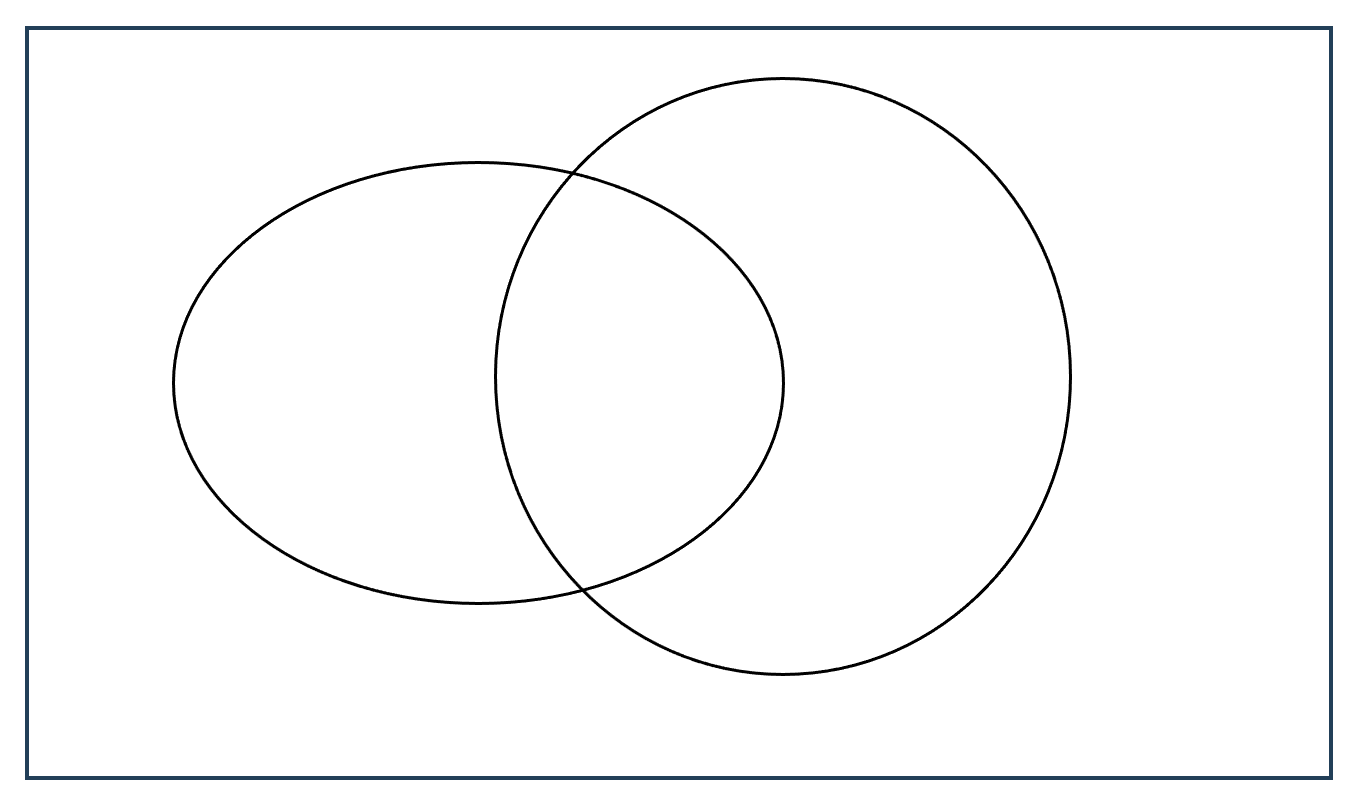
\includegraphics[scale=.3]{figs/VDblankTwoSets1.png} 
  	\end{center}
	\vspace{4in}
	\end{frame}
	
\begin{frame}
 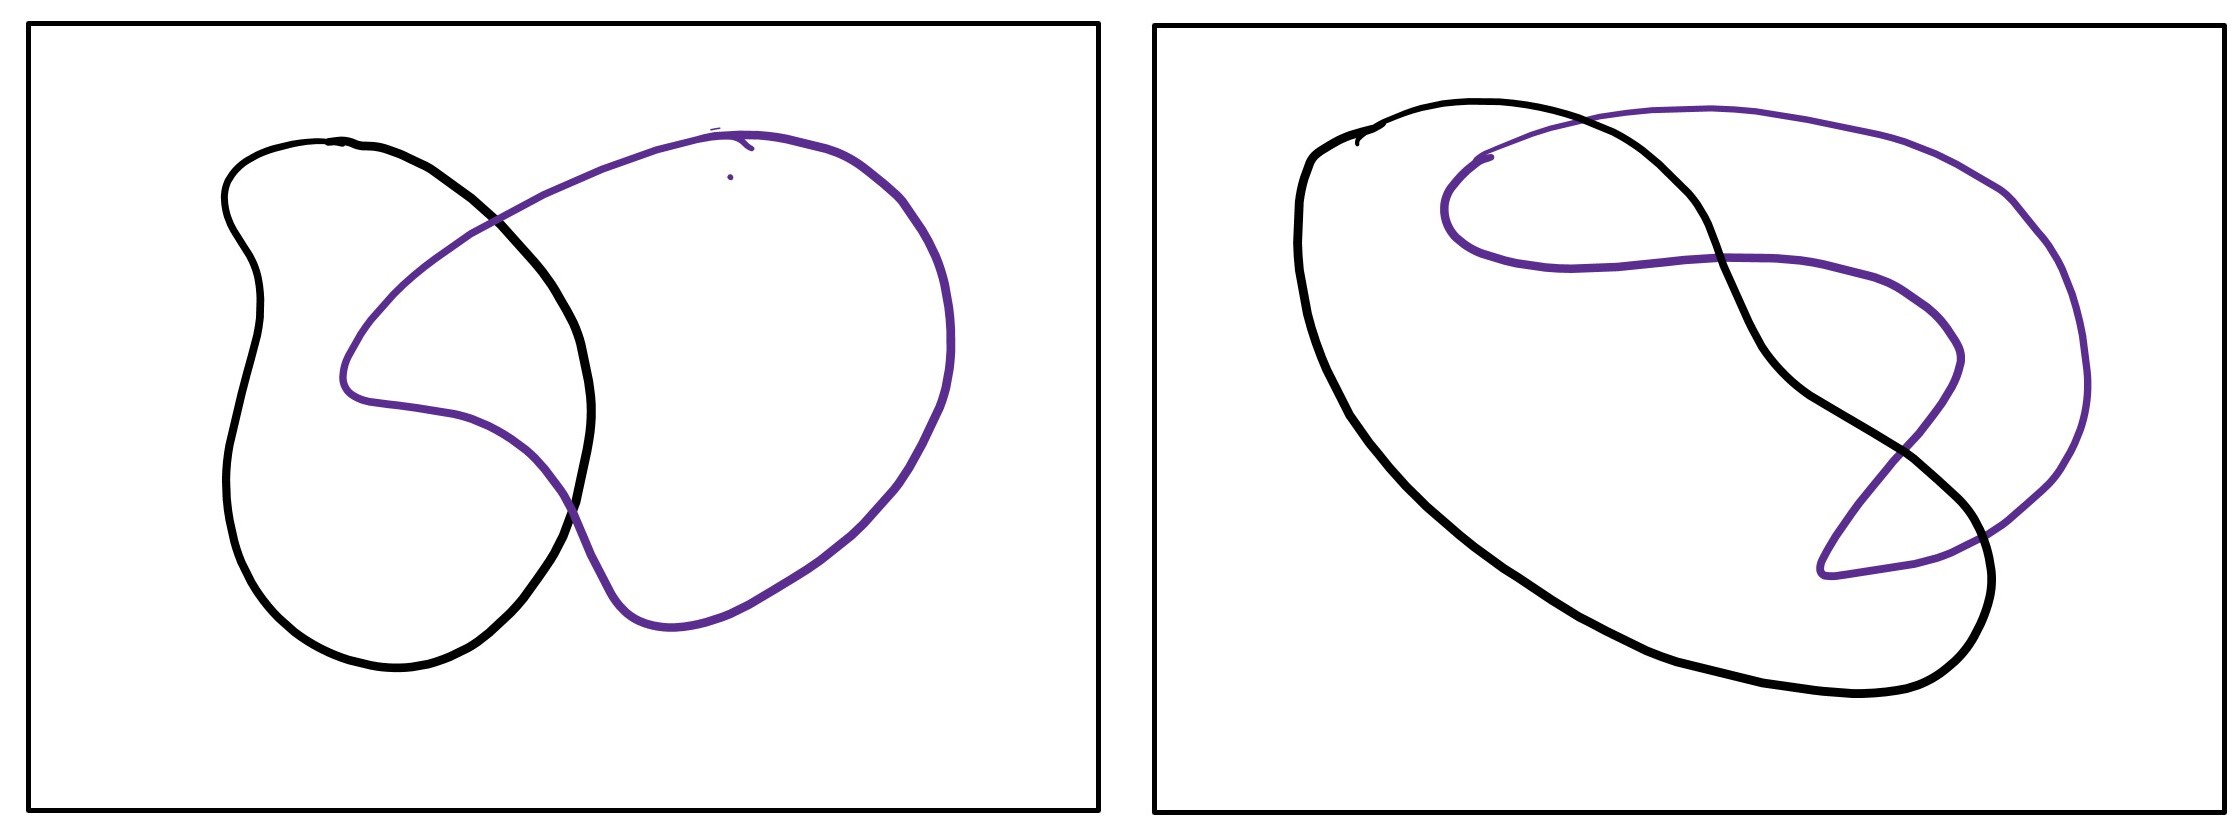
\includegraphics[scale=.36]{figs/BlankVD1.jpg} 
  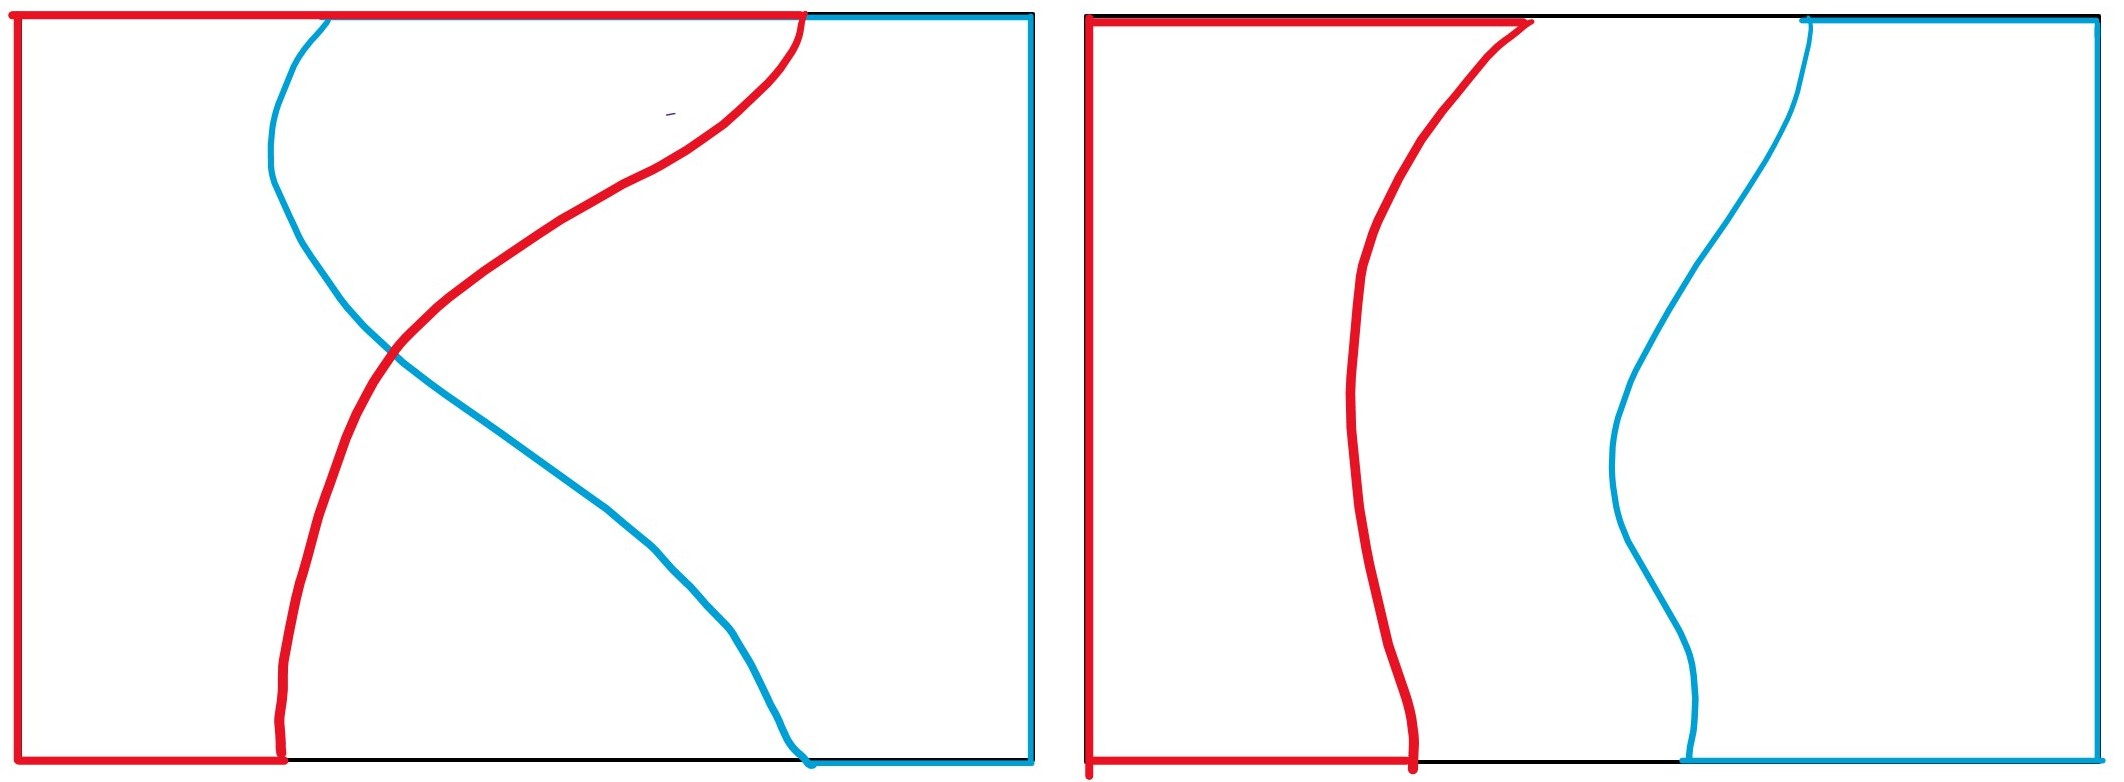
\includegraphics[scale=.38]{figs/BlankVD3.jpg} 
\end{frame}	
	
	
	
	
	
	
	\begin{frame}
	\frametitle{Set Operation: Intersection}
		\vspace{-.1in}
	\begin{center}
\qbx[4.2in]{applegreen!40}{\qBrd[1.2in]{teal!30}{\bf A Intersection B:}  A Intersection B,  denoted by  $\HLTY{A \cap B}$ is the set of all elements that are  both $A$ and $B$.\\
}\\
\pause
\vspace{-.2in}
  \qbx[3in]{asparagus!60}{  
 The logical operator is \HLTY{\text{AND} }.
  }
   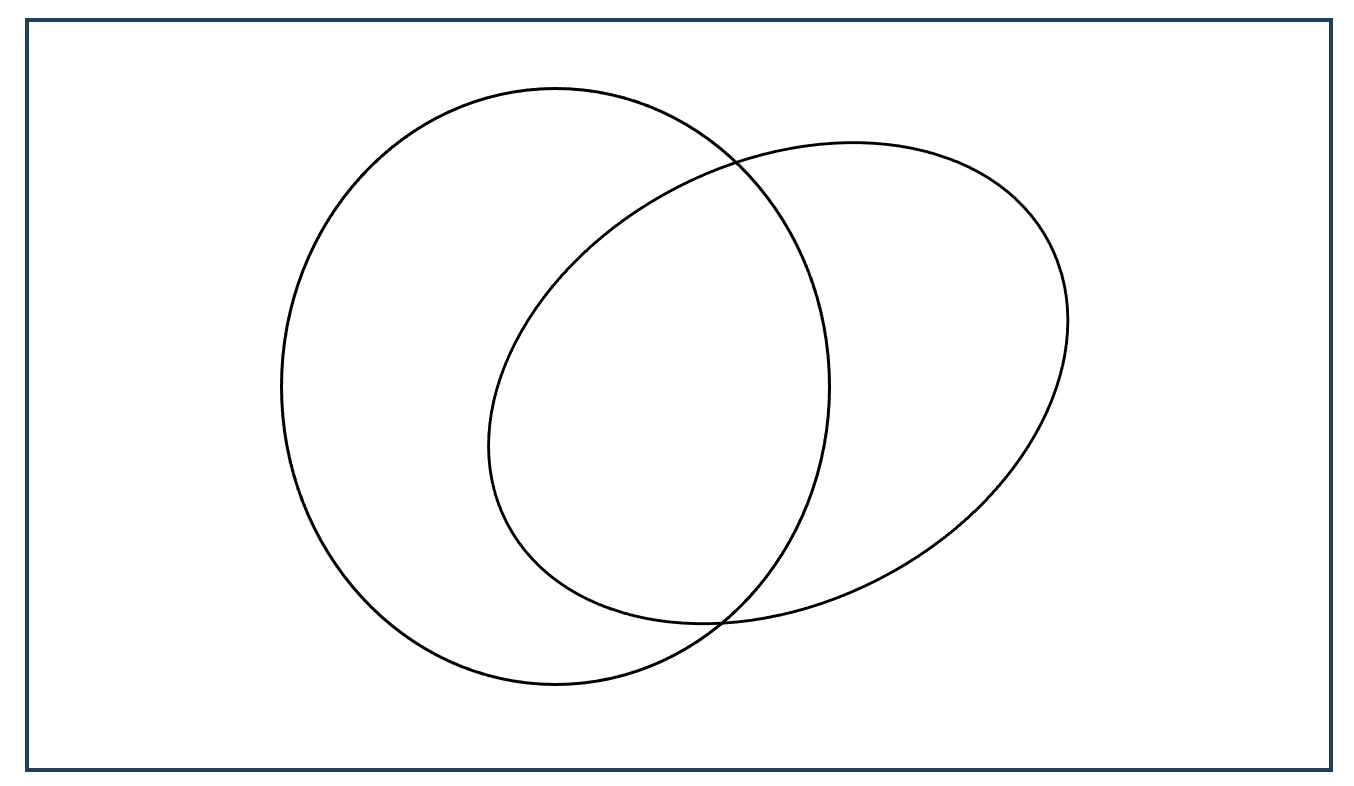
\includegraphics[scale=.3]{figs/VDblankTwoSets2.png} 
  	\end{center}
	\vspace{4in}
	\end{frame}
	


\begin{frame}
 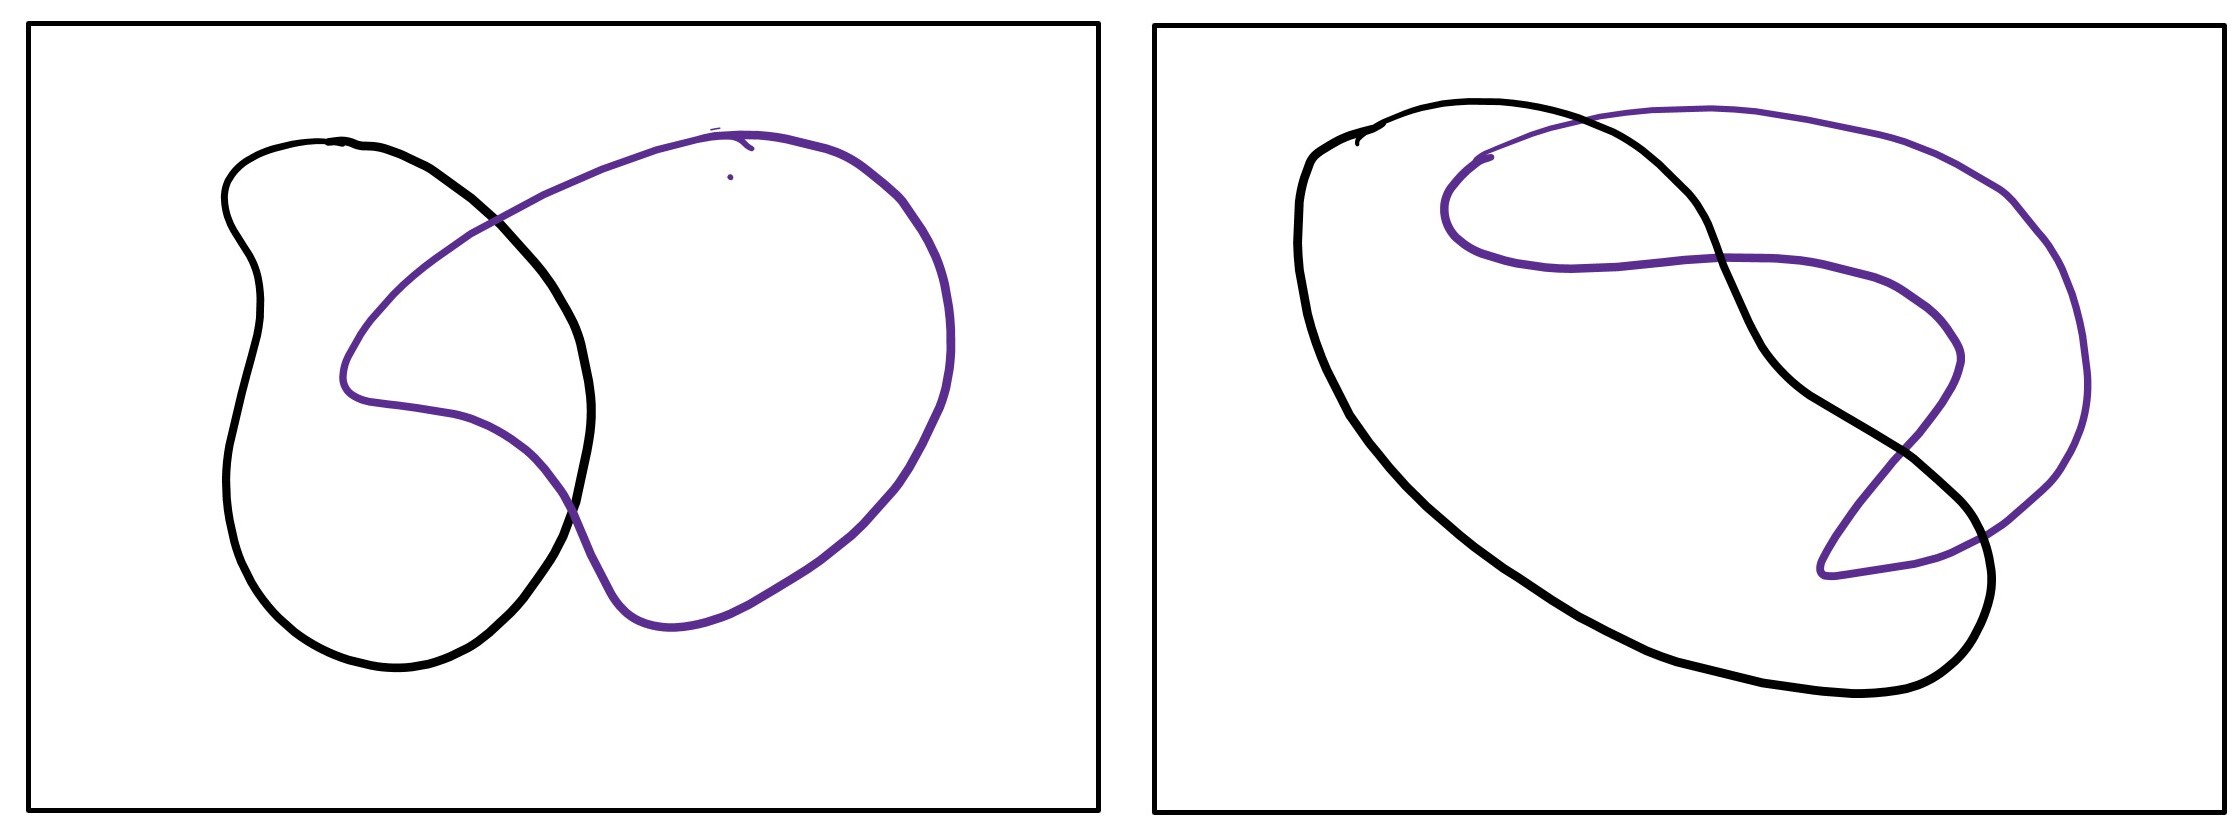
\includegraphics[scale=.36]{figs/BlankVD1.jpg} 
 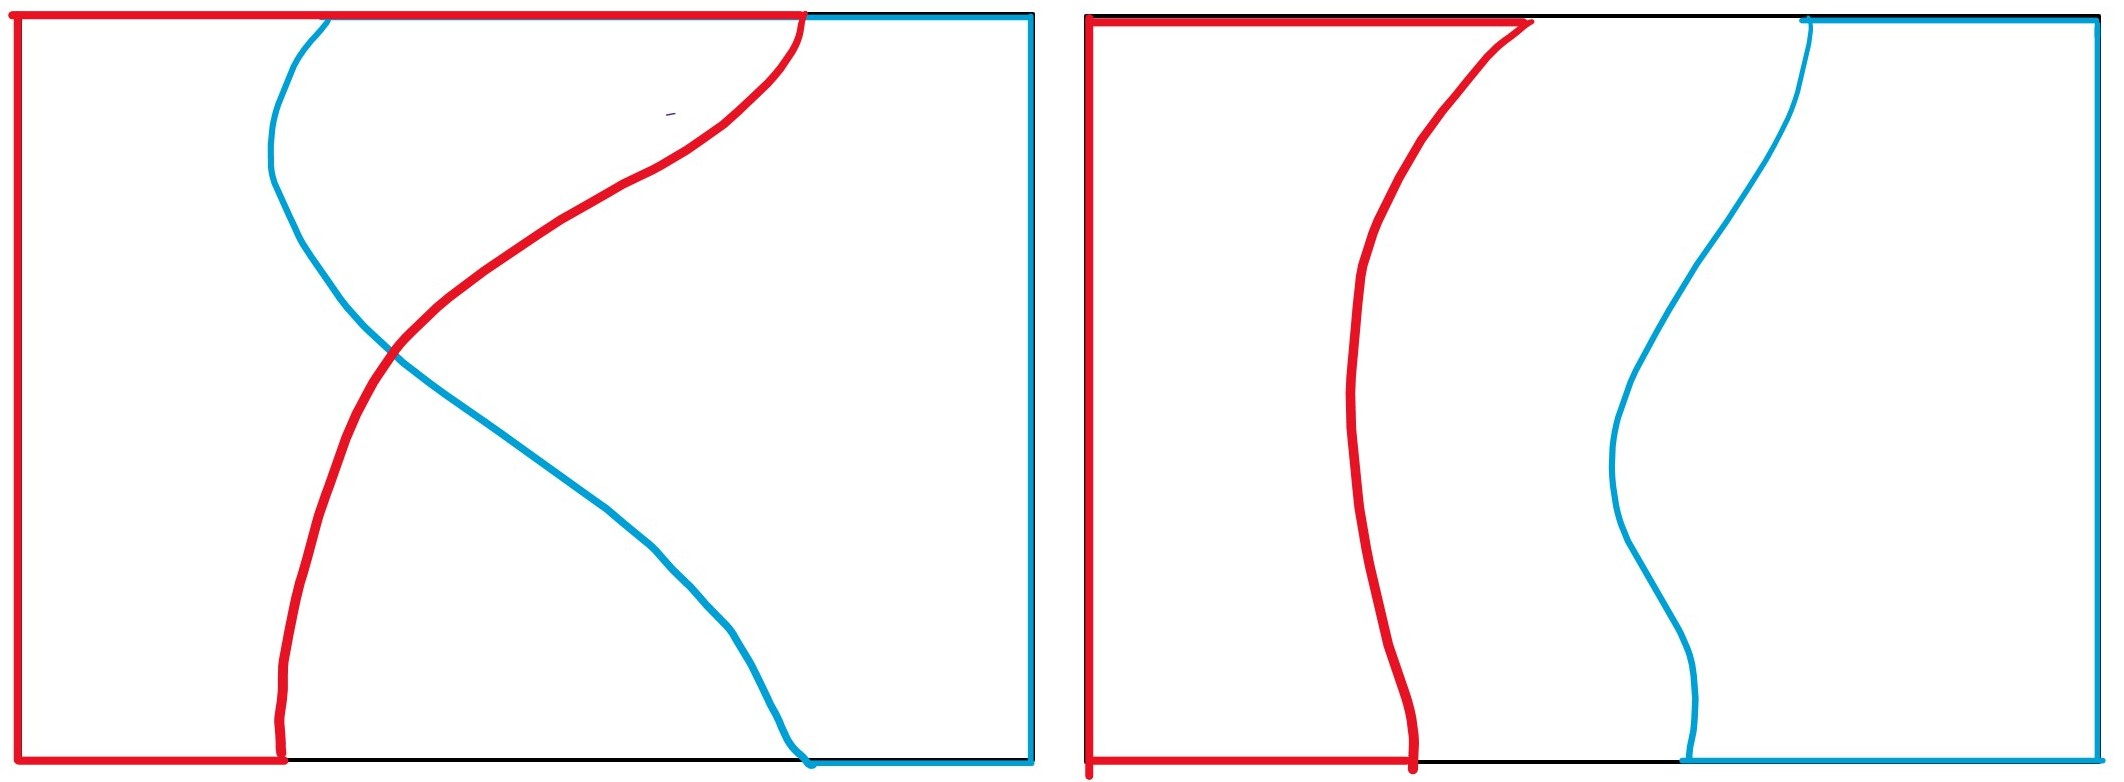
\includegraphics[scale=.38]{figs/BlankVD3.jpg} 
\end{frame}	
	
	
	
	
	\begin{frame}
	\frametitle{Set Operation: Complement}
		\vspace{-.1in}
	\begin{center}
\qbx[4.2in]{applegreen!40}{\qBrd[1.2in]{teal!30}{\bf A Complement :}  A Complement,  denoted by  $\HLTY{\Not{A}}$ is the set of all elements that are  not in  $A$. {\tiny Sometimes it is also denoted by $A^c$}\\
}\\
\pause
\vspace{-.2in}
  \qbx[3in]{asparagus!60}{  
 The logical operator is \HLTY{\text{NOT} }.
  }
    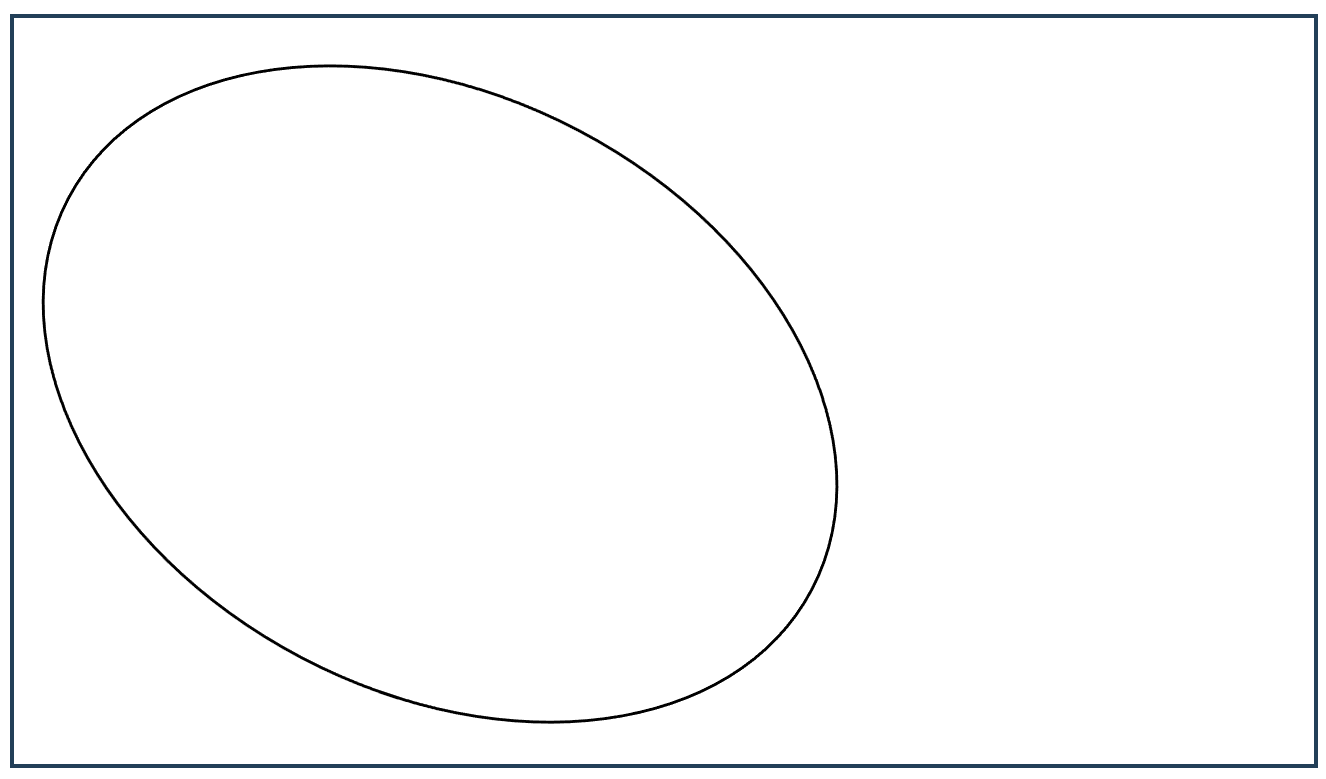
\includegraphics[scale=.22]{figs/VDblankOneSets1.png} 
     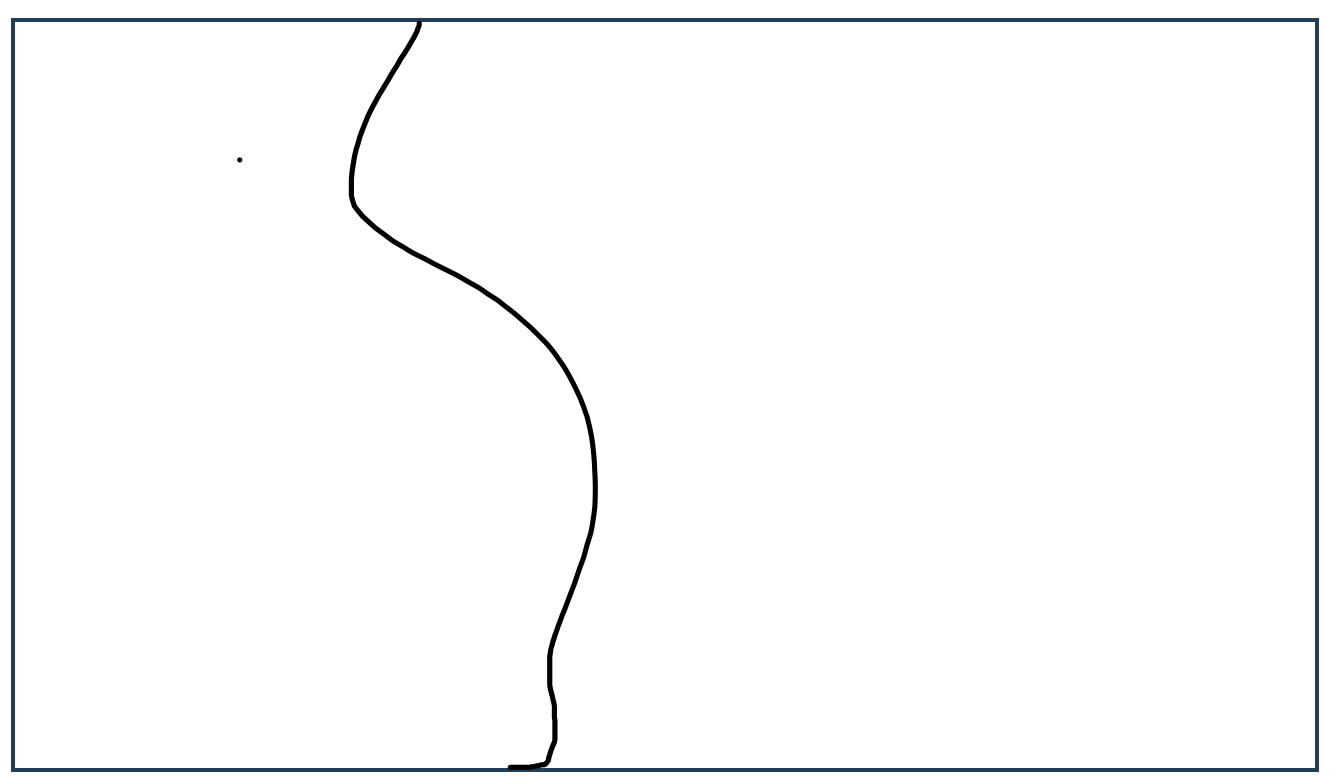
\includegraphics[scale=.22]{figs/VDblankOneSets2.png} 
  	\end{center}
	\vspace{4in}
	\end{frame}



\begin{frame}
	\frametitle{Set Operation: Set Difference}
		\vspace{-.1in}
	\begin{center}
\qbx[4.3in]{teal!30}{\qBrd[1in]{olive!30}{\bf A Minus B:}  A Minus B,  denoted by  $\HLTY{A - B}$ is the set of all elements that are only an element of $A$, but not an element of the set $ B$.
}\\
\pause
\vspace{-.2in}
  \qbx[3in]{applegreen!50}{  
 $\HLTY{A-B}$ is same as: $ \HLTY{A \cap \Not{B} }$.
  }
  
  {\tiny {\bf Comment:} $\HLTY{A-B}$ is not same as $\HLTY{B-A}$ }
  	\end{center}
  	 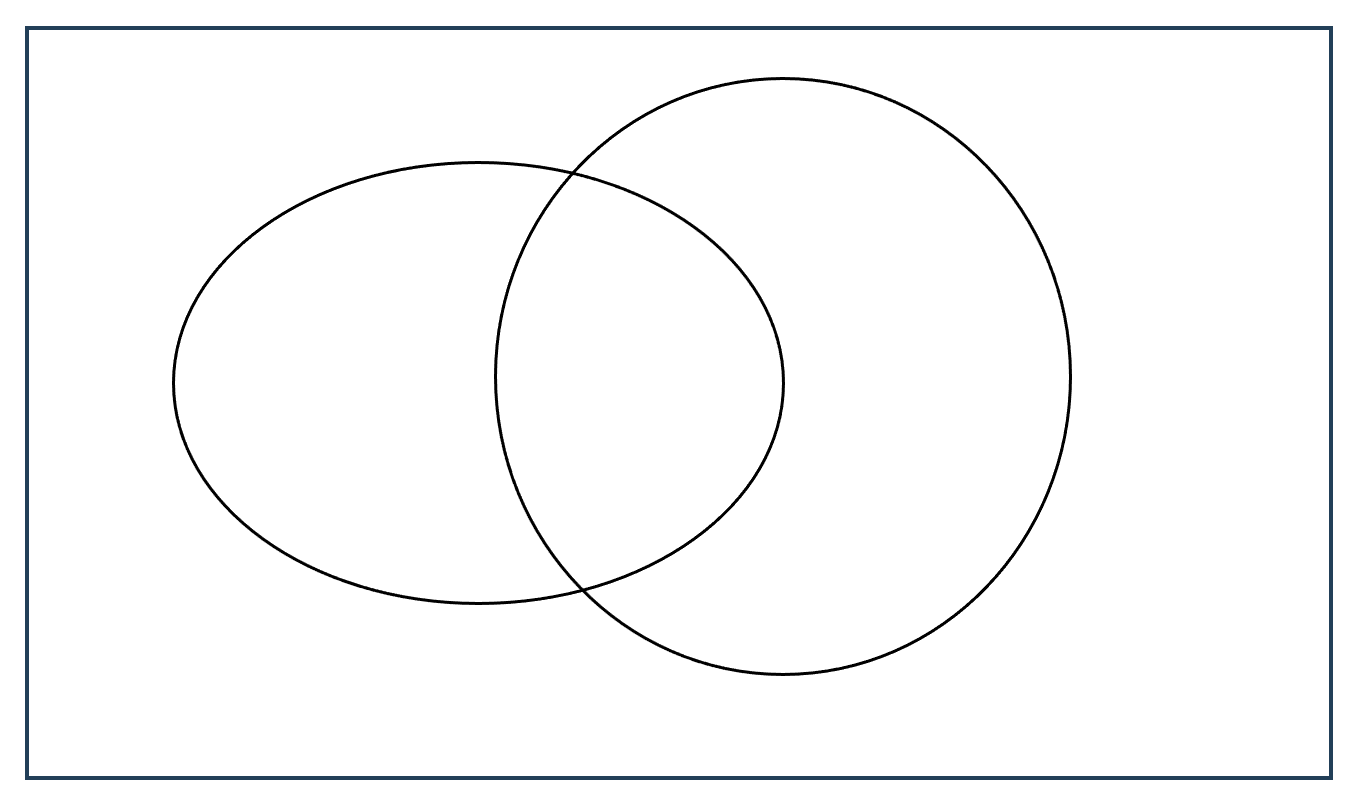
\includegraphics[scale=.2]{figs/VDblankTwoSets1.png} 
  	  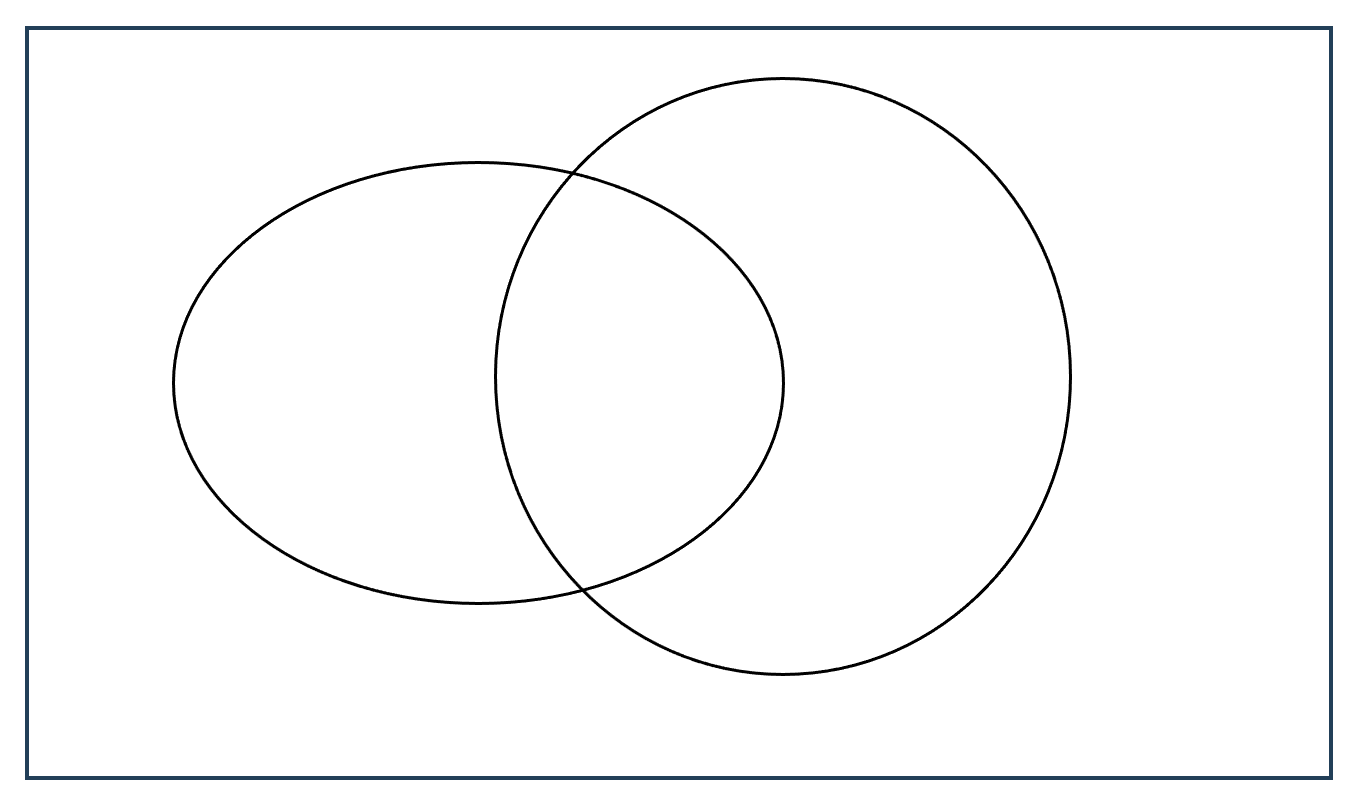
\includegraphics[scale=.2]{figs/VDblankTwoSets1.png} 
	\vspace{4in}
	\end{frame}



\begin{frame}
	\frametitle{A Few Rules for Various  Set Operations}
	
	\qbx[4in]{blue!40}{
\begin{itemize}
\item[]\qBrd[3in]{babyblue!40}{ $A \cup\left( B\cup C\right)= \left(A \cup B\right)\cup C= A \cup B\cup C $}
\item[]  \qBrd[3in]{babyblue!70}{$A \cap\left( B\cap C\right)= \left(A \cap B\right)\cap C= A \cap B\cap C $}
\end{itemize}	
}
\vspace{.05in}

	\qbx[4in]{amethyst!70}{
	\HLTY{\text{\it \small Distributive laws of Union \& Intersection}}
\begin{itemize}
\item[] \qBrd[2.5in]{blush!40}{$A \cap\left( B\cup C\right)= \left(A \cap B\right)\cup \left(  A \cap C \right)$}
\item[] \qBrd[2.5in]{blush!60}{ $A \cup\left( B\cap C\right)= \left(A \cup B\right)\cap \left(  A \cup C \right)$}
\end{itemize}	
}
\vspace{.1in}

	\qbx[4in]{asparagus!80}{
	\HLTY{\text{\small \it DeMorgan's laws}}
\begin{itemize}
\item[] \qBrd[2.1in]{applegreen!40}{$\Not{\left( A\cap B\right)}= \left(\Not{A} \cup \Not{B}\right)$}
\item[] \qBrd[2.1in]{applegreen!60}{$\Not{\left( A\cup B\right)}= \left(\Not{A} \cap \Not{B}\right)$}
\end{itemize}	
}
	
	\end{frame}







\begin{frame}
	\frametitle{Set Operation: Examples}
	
\end{frame}

\section{A Few  Examples  Using Venn Diagrams}
\TransitionFrame[antiquefuchsia]{\Large A Few  Examples  Using Venn Diagrams }
\begin{frame}
  \qbx[4.4in]{applegreen!50}{ \sqBullet{olive}  {\bf Venn Diagrams} are graphical representation of the sets that are typically used to depict the relation between various sets  }
  \vspace{3in}
\end{frame}


%\TransitionFrame[antiquefuchsia]{\Large Venn Diagrams: Examples}
\begin{frame}\frametitle{Venn Diagrams: Examples}
  \begin{center}
 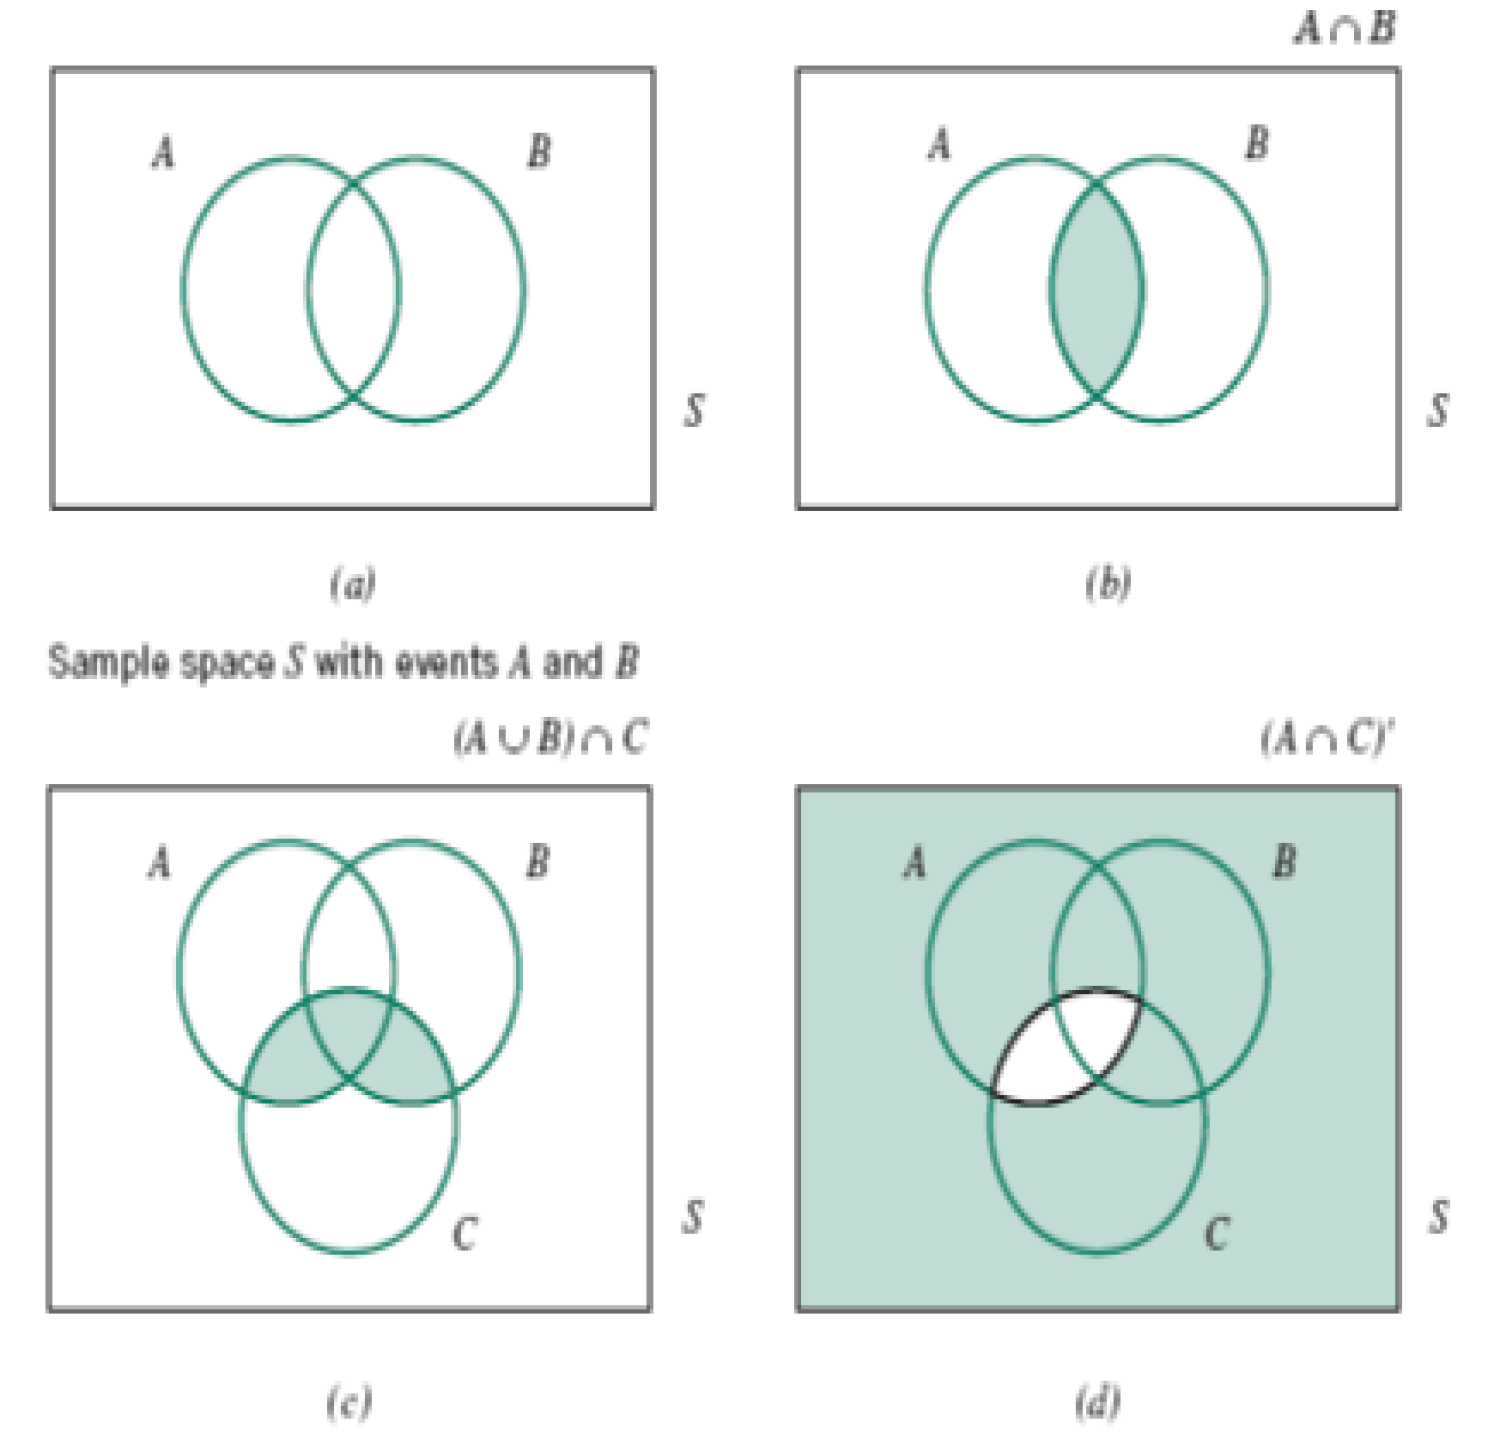
\includegraphics[scale=.32]{figs/VennDiagram1.png}
 \end{center} 
\end{frame}



%\TransitionFrame[antiquefuchsia]{\Large Venn Diagrams: Examples}
\begin{frame}\frametitle{Venn Diagrams: Examples}
  \begin{center}
  \qBrd[4.1in]{olive!30}{ Let $\SampleS= \{1,2,3,4,5,6,7,8\}$,\\
   $A=\{1,2,6,7\}$,  $B=\{ 2,3,4,7 \}$,  and $C=\{4,5,6,7\}$ }
 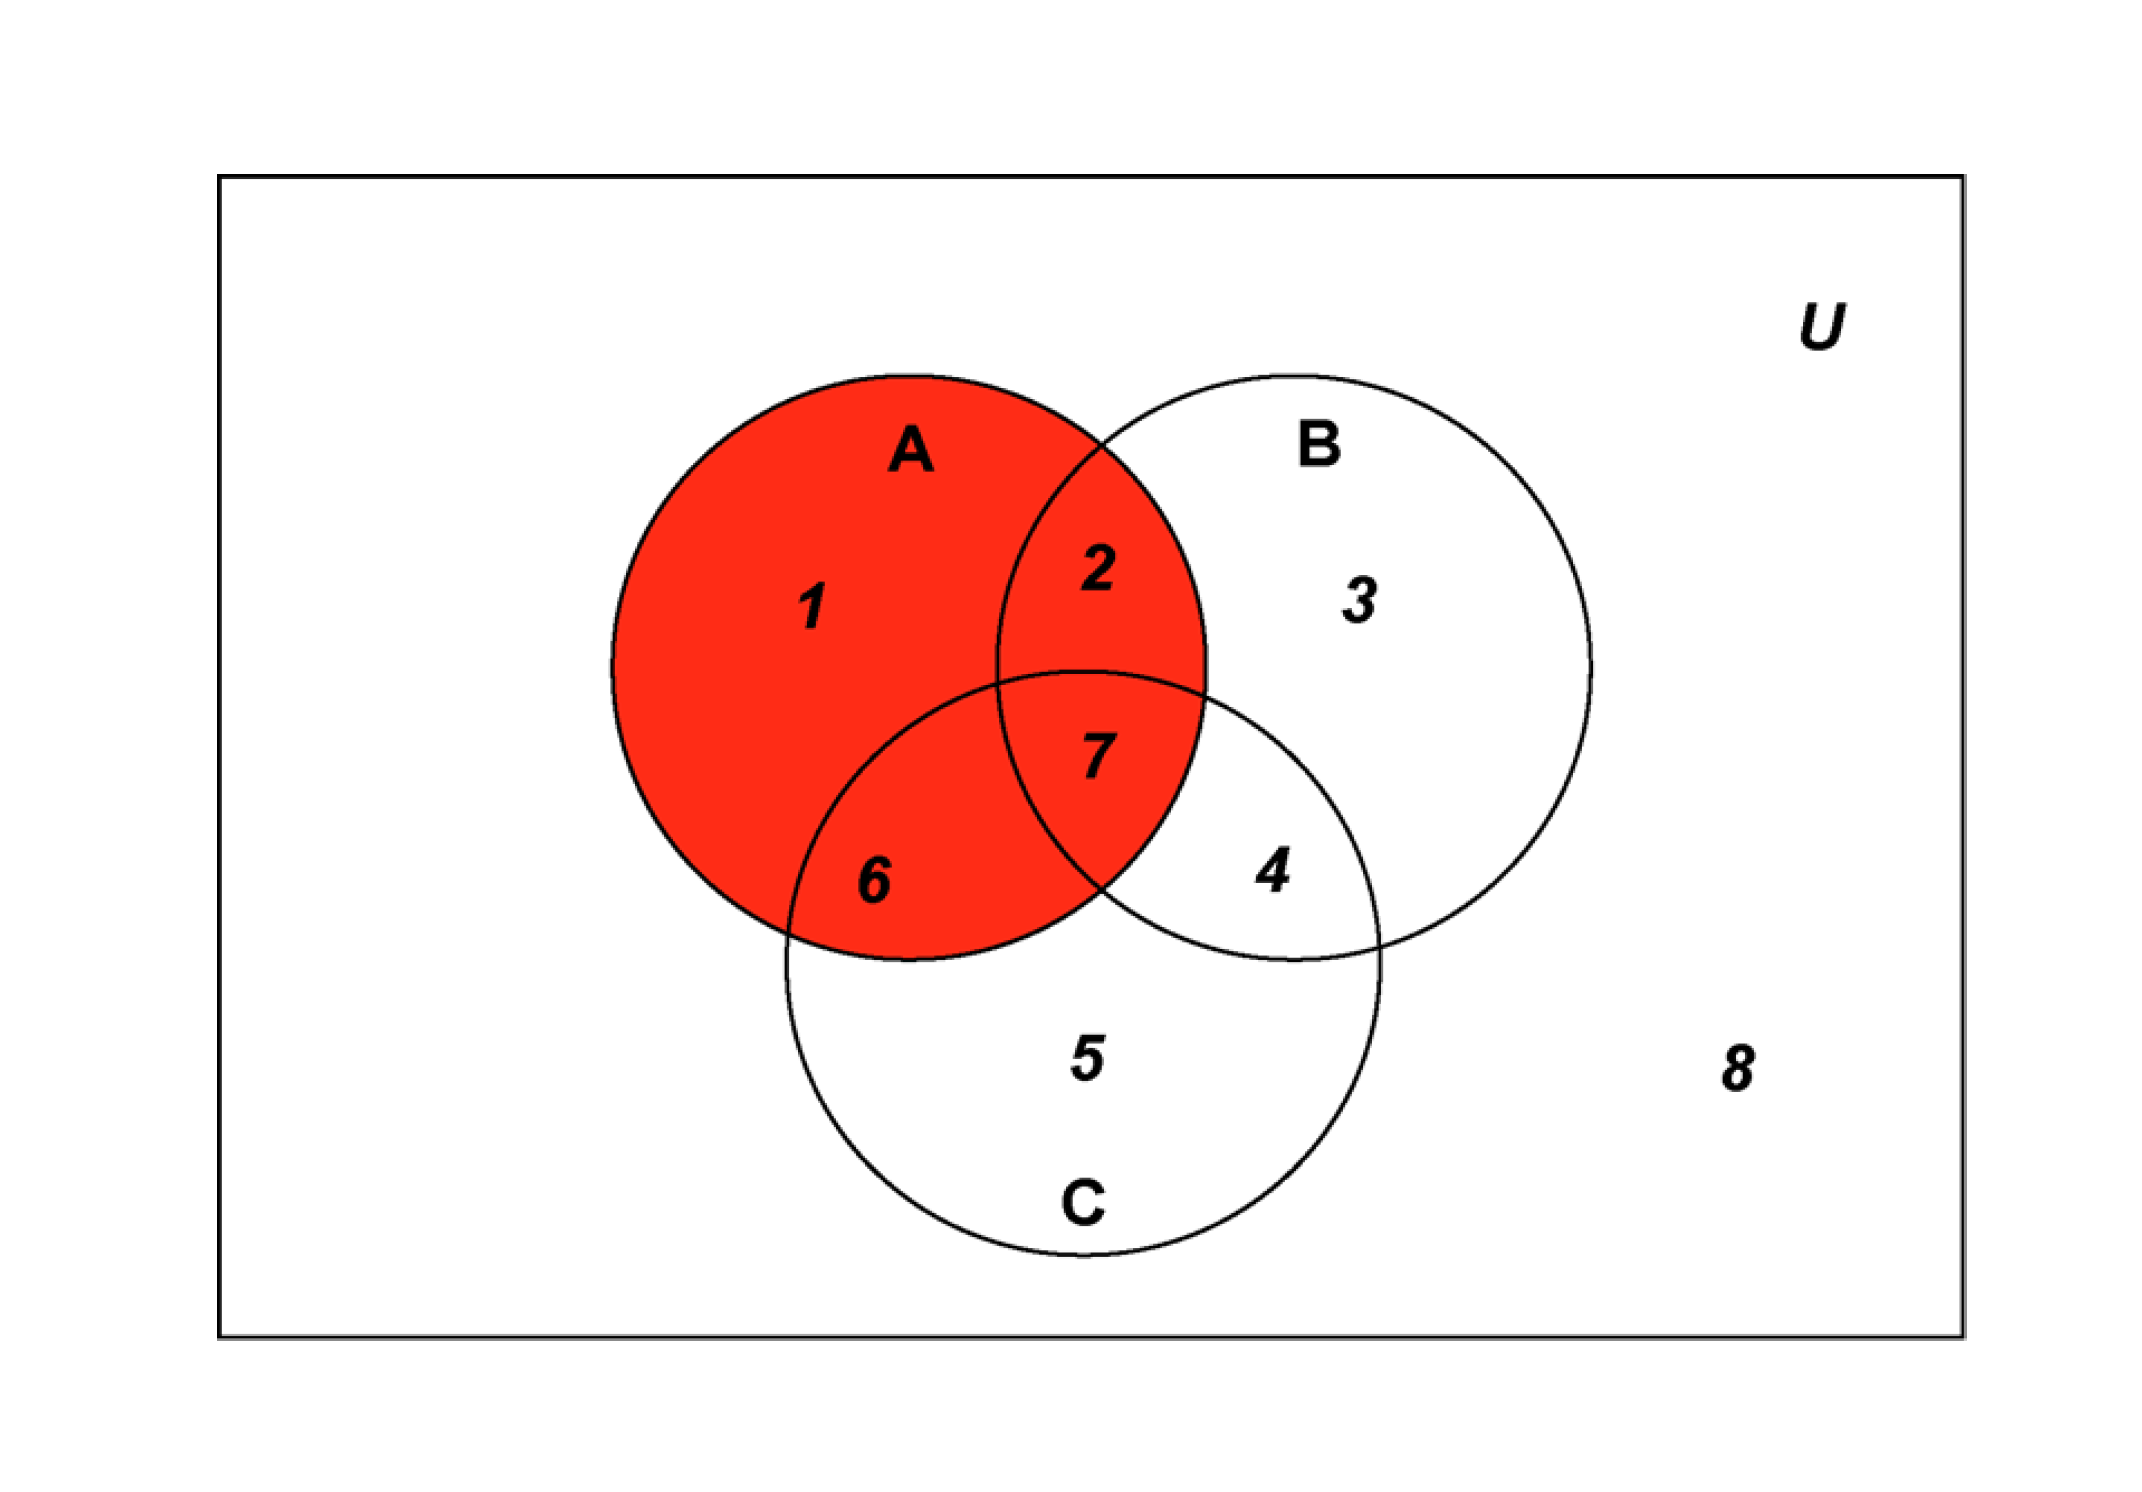
\includegraphics[scale=.26]{figs/VennDiagram2.png}
 \end{center} 
\end{frame}





\section{Disjoint Sets \& Partition }
\TransitionFrame[wisteria]{\Large Disjoint Sets \& Partition  }



\begin{frame}
	\frametitle{Disjoint Sets}
	\vspace{-.1in}
	\begin{center}
\qbx[4.3in]{teal!30}{\qBrd[1in]{olive!30}{\bf Disjoint Sets:}  Two sets  A, and  B are said to be  {\bf Disjoint Sets} or {\bf mutually exclusive sets} if $A$ and $B$ does not have any elements in common.\\
}\\
\pause
\vspace{-.2in}
  \qbx[3in]{applegreen!50}{  
 A and B are Disjoint $\Leftrightarrow \HLTY{A\cap B=\emptyset}$.
  }
  
  	\end{center}
	\vspace{4in}
	\end{frame}


\begin{frame}
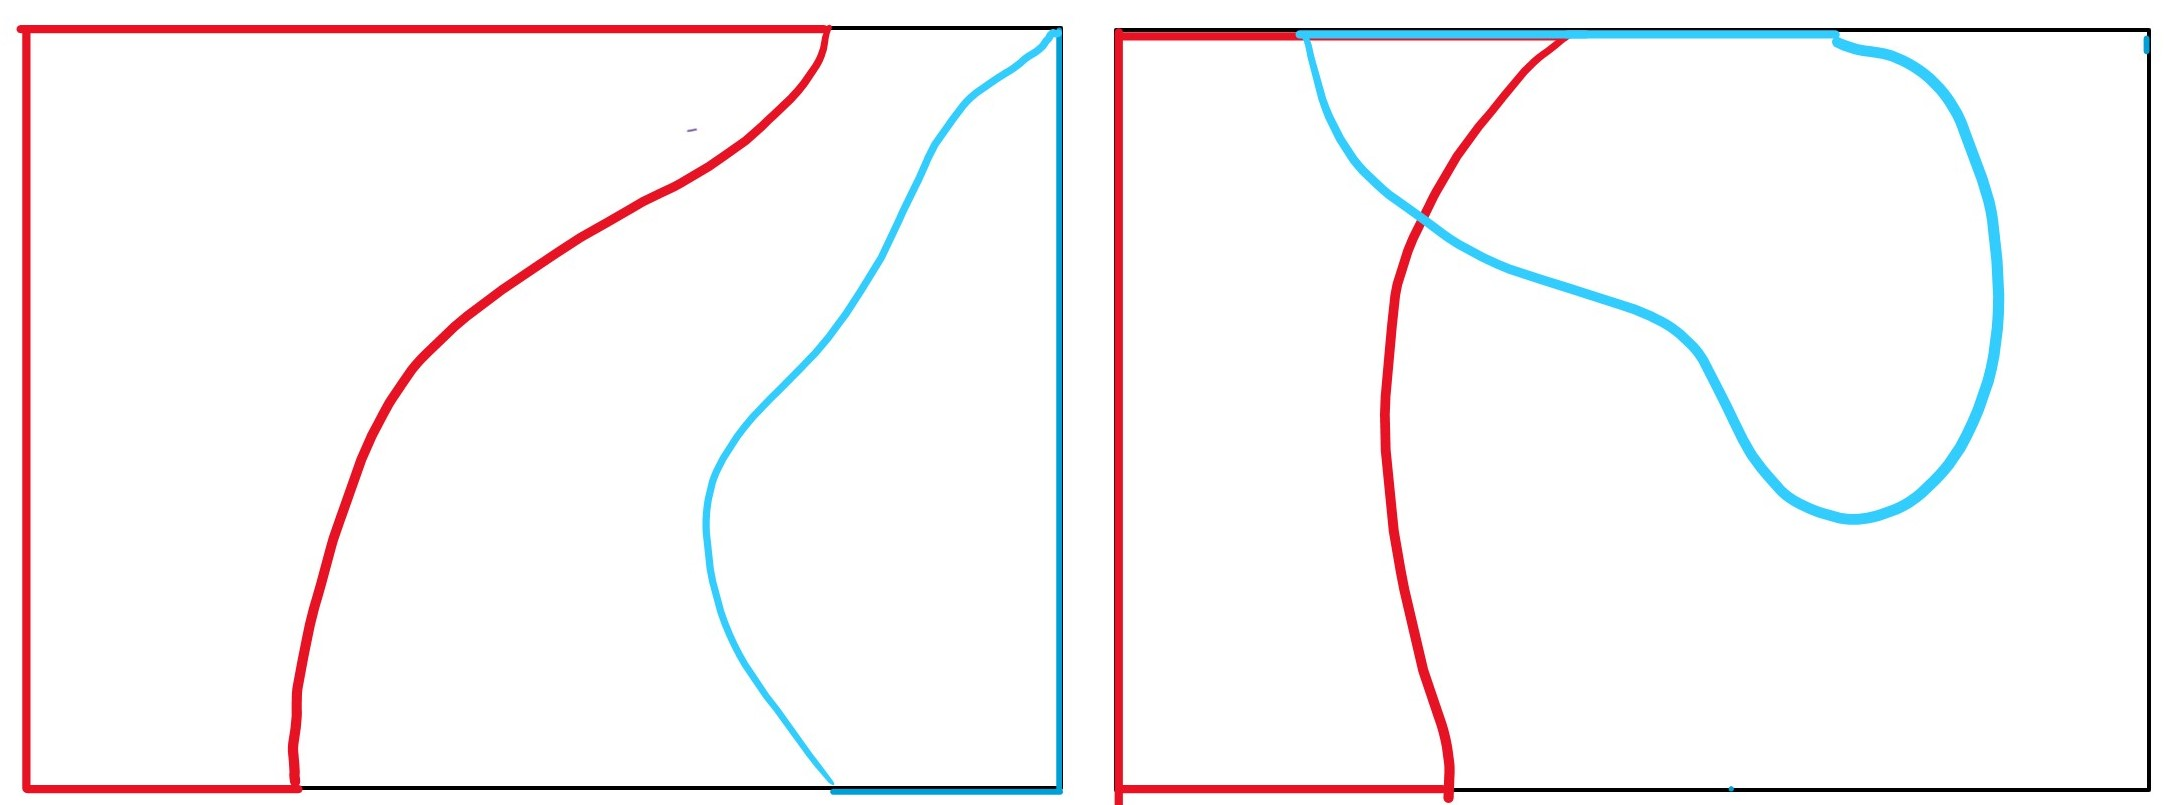
\includegraphics[scale=.35]{figs/BlankVD4.jpg} 
  	  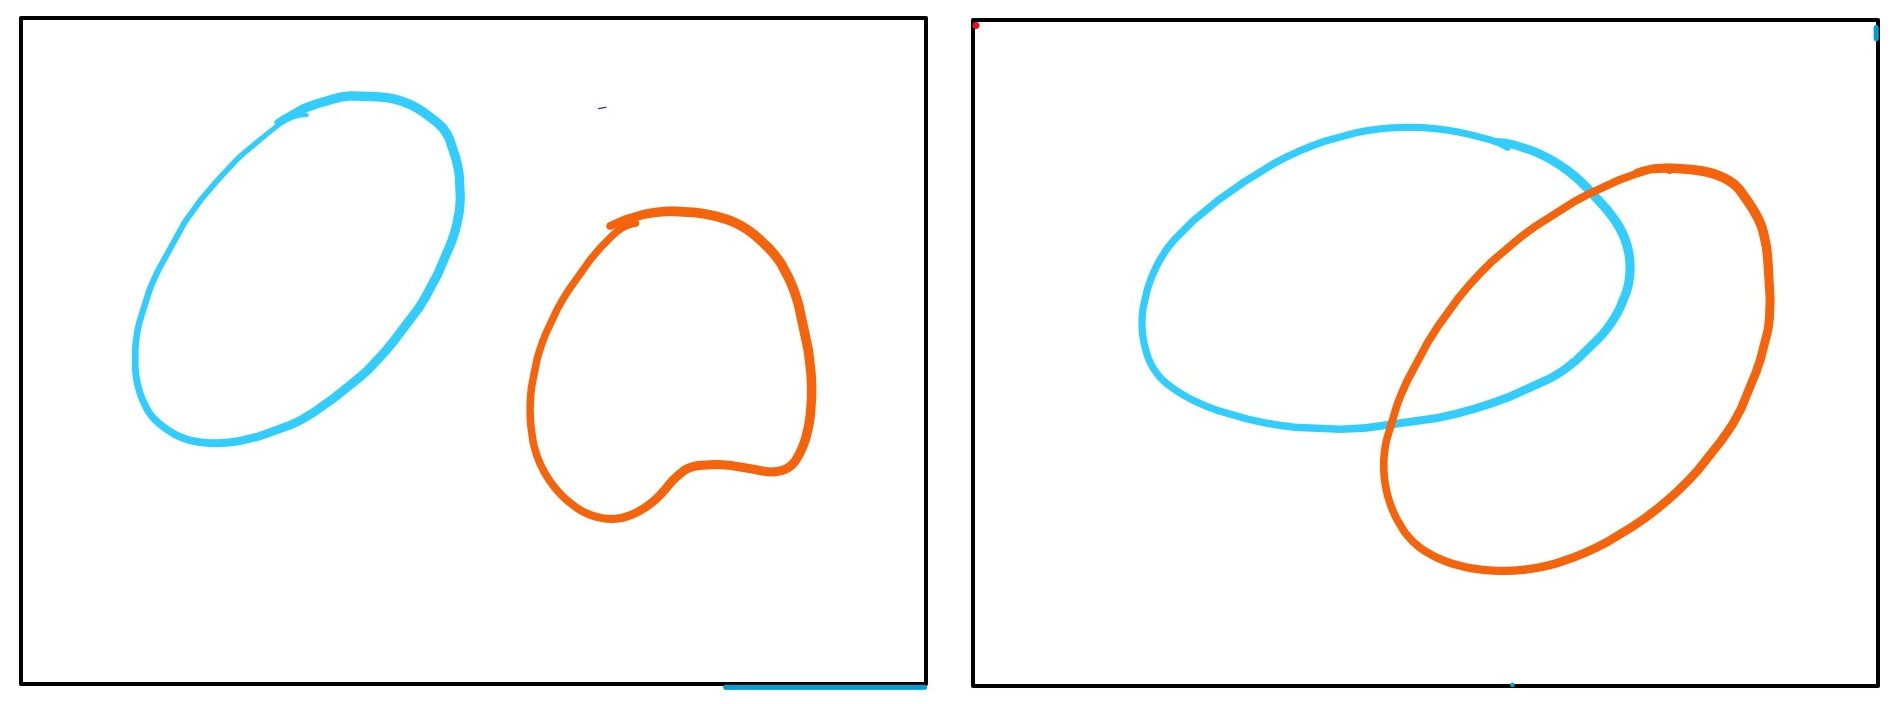
\includegraphics[scale=.4]{figs/BlankVD5.jpg} 
\end{frame}







\begin{frame}
	\frametitle{Exhaustive}
	\vspace{-.1in}
	\begin{center}
\qbx[4.3in]{babyblueeyes!50}{\qBrd[1in]{blue!30}{\bf Exhaustive:}  A collection of sets  $A_1$,  $A_2, \cdots, A_k$ are exhaustive for the set  $\HLTW{C}$ if $\HLTY{A_1\cup A_2\cup \cdots \cup  A_k} =\HLTW{C}$.\\
}\\
\vspace{-.2in}
  \qbx[3.4in]{applegreen!50}{  
 A and B are exhaustive for C $\Leftrightarrow \HLTY{\displaystyle \bigcup_{i=1}^{k}A_i}=\HLTW{C}$.
  }
  
  	\end{center}
  	
	\vspace{4in}
	\end{frame}
	
	
	\begin{frame}
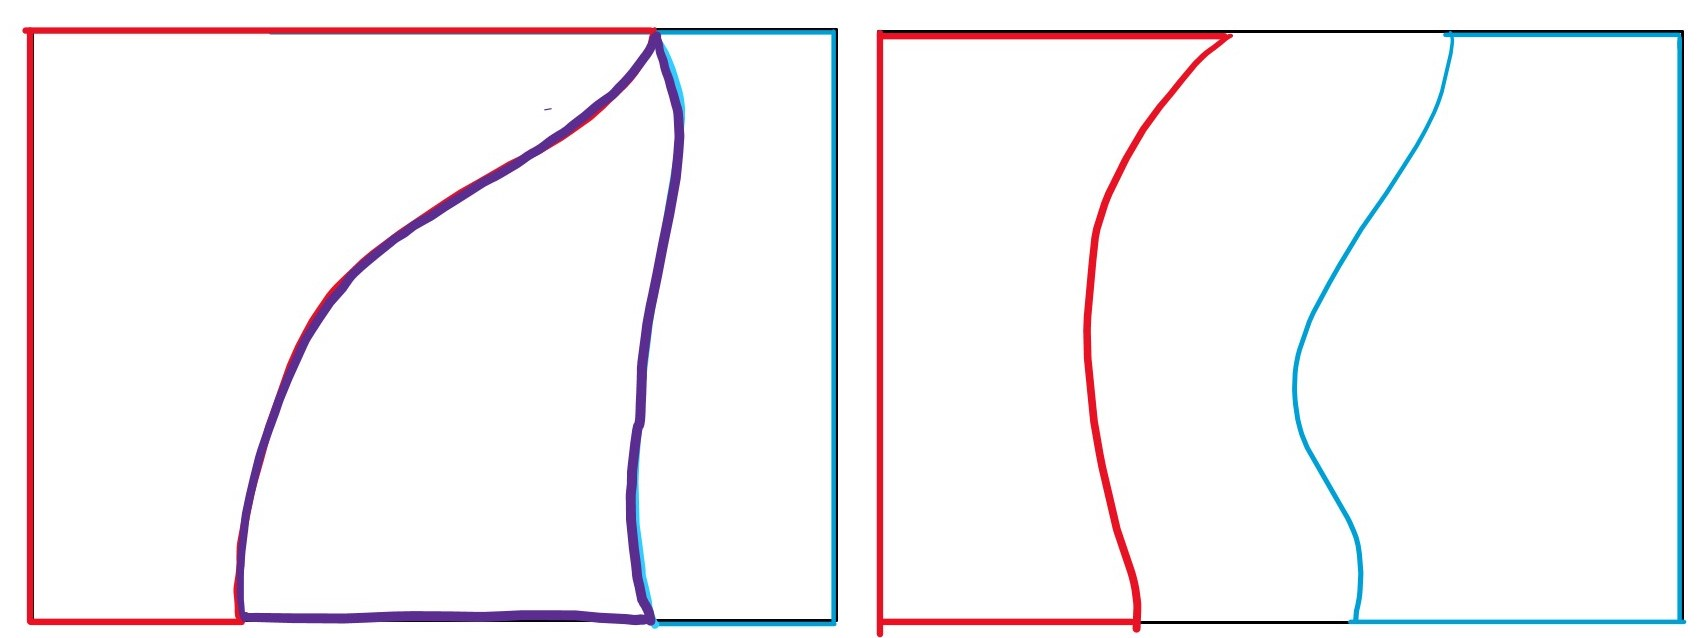
\includegraphics[scale=.4]{figs/BlankVD6.jpg} 
  	 % 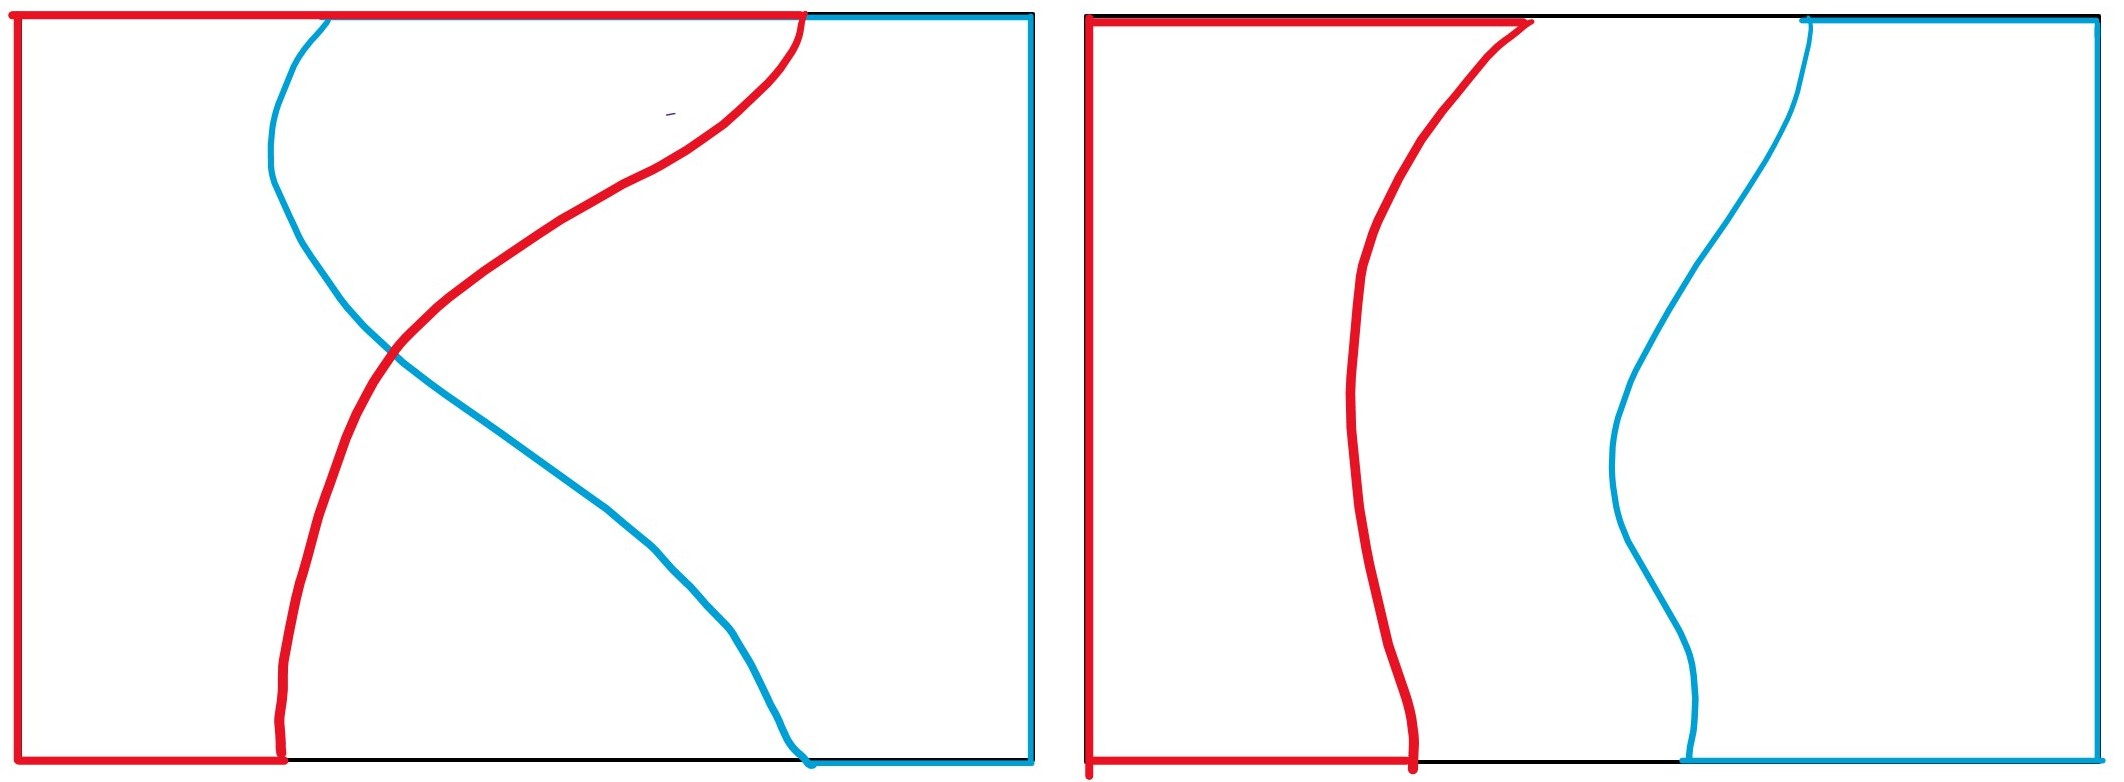
\includegraphics[scale=.4]{figs/BlankVD3.jpg} 
\end{frame}
	
	
	
	
	

\begin{frame}
	\frametitle{Exhaustive: Special Case}
	\vspace{-.1in}
	\begin{center}
\qbx[4.3in]{babyblueeyes!50}{\qBrd[1in]{blue!30}{\bf Exhaustive:}  Two sets A and B are exhaustive for the set  C if $A\cup B =C$.\\
}\\
\vspace{-.2in}
  \qbx[3in]{applegreen!50}{  
 A and B are exhaustive for C $\Leftrightarrow \HLTY{A\cup B}=C$.
  }
  
  	\end{center}
  	
	\vspace{4in}
	\end{frame}
	
	
	\begin{frame}
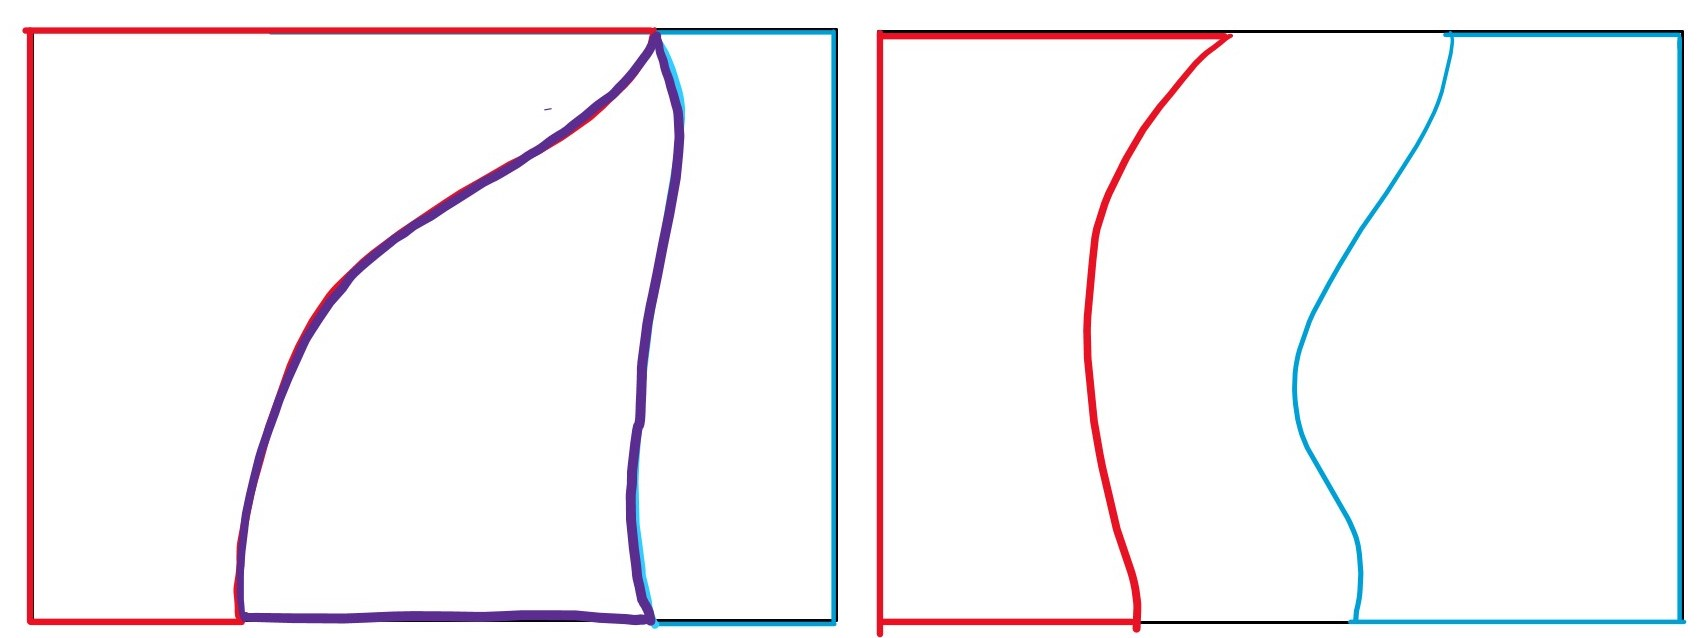
\includegraphics[scale=.4]{figs/BlankVD6.jpg} 
  	 % 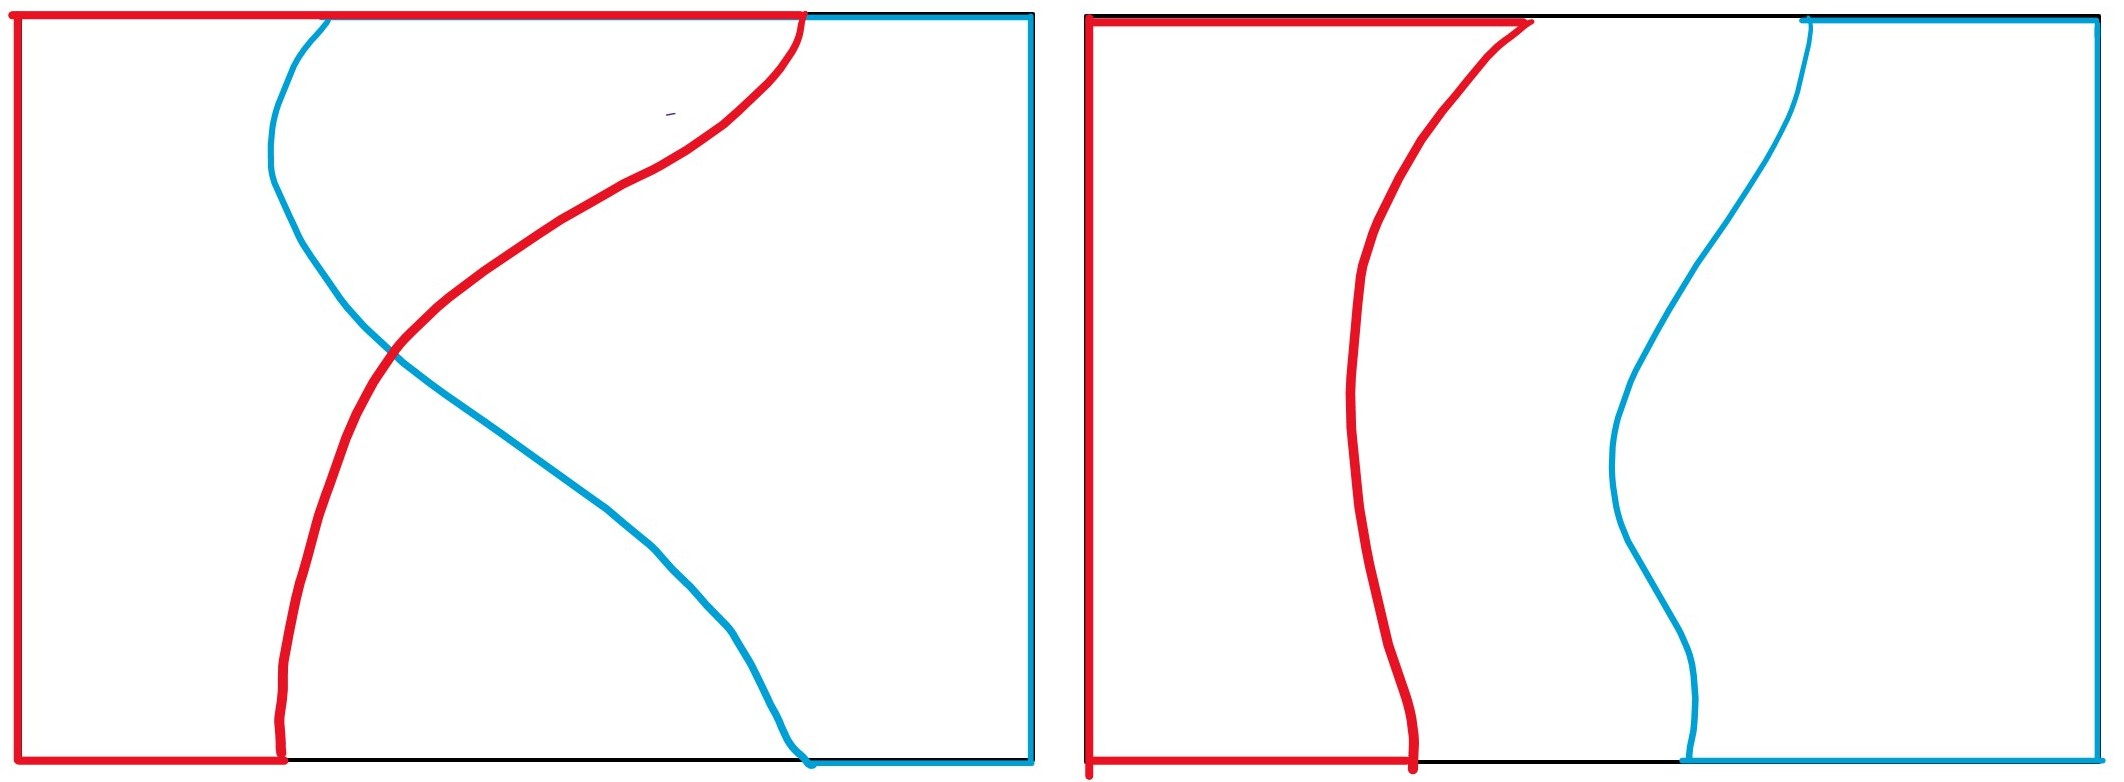
\includegraphics[scale=.4]{figs/BlankVD3.jpg} 
\end{frame}
		
	

\begin{frame}
	\frametitle{Partition}
	\begin{center}
\qbx[4.6in]{antiquebrass!60}{\qBrd[1in]{olive!30}{\bf Partition:}  A collection of sets $\HLTY{\{A_1, A_2, \cdots, A_k\}}$ is called a {\bf partition for a set $\HLTW{C}$} if
\begin{enumerate}
\item  \qBrd[3.5in]{applegreen!30}{$A_i \cap A_j = \emptyset$ for $1\leq i \neq j \leq k$ ({\tiny  i.e. ,$A_i$,  and $A_j$ are Disjoint if $i\neq j$}) }, and 
\item  \qBrd[4in]{teal!30}{$\HLTY{A_1\cup A_2\cup \cdots \cup  A_k} =\HLTW{C}$ ({\tiny i.e. , A and B is exhaustive for C}).}
\end{enumerate}
}\\
\pause
  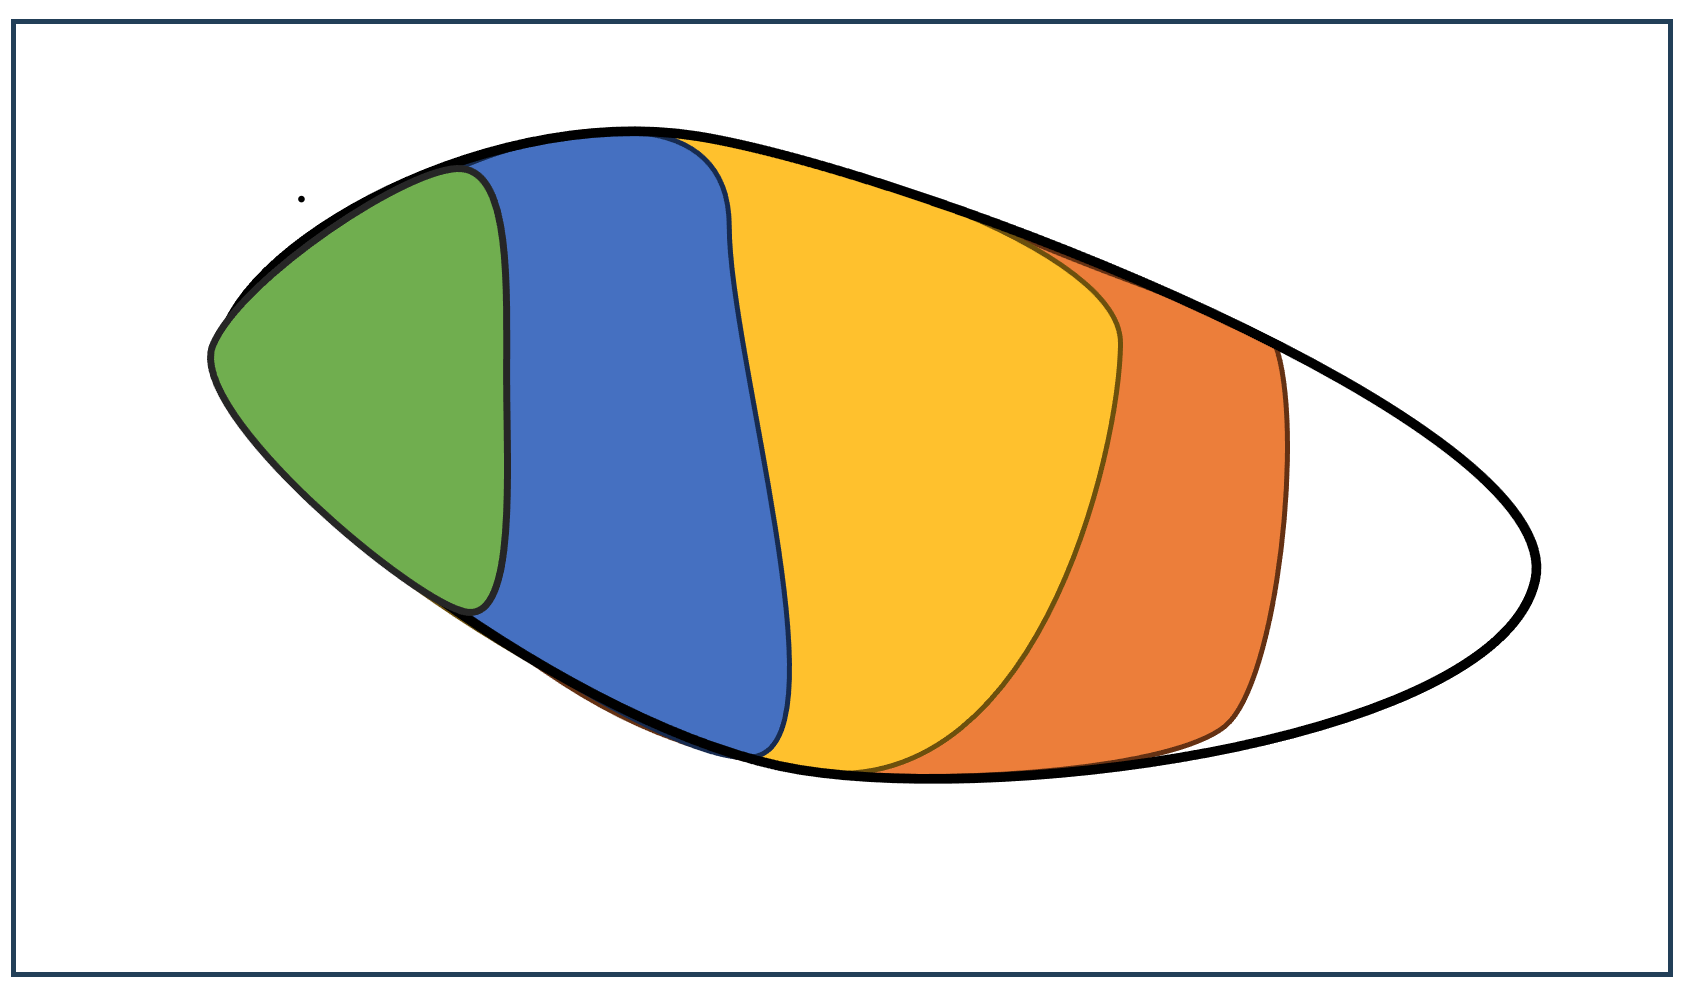
\includegraphics[scale=.2]{figs/VDPartition2.png} 
  	\end{center}
  	
	\vspace{4in}
	\end{frame}
	
	
	

\begin{frame}
	\frametitle{Partition: Special Case }
	\begin{center}
\qbx[4.3in]{antiquebrass!60}{\qBrd[1in]{olive!30}{\bf Partition:}  A group of sets $\{A, B\}$ is called a {\bf partition for a set $\HLTY{C}$} if
\begin{enumerate}
\item  \qBrd[2.5in]{applegreen!30}{$A\cap B = \emptyset$ ( i.e. ,$A$,  and $B$ are Disjoint) }, and 
\item  \qBrd[3.5in]{teal!30}{$A\cup B= \HLTY{C}$ (i.e. , A and B is exhaustive for C).}
\end{enumerate}
}\\
\pause
  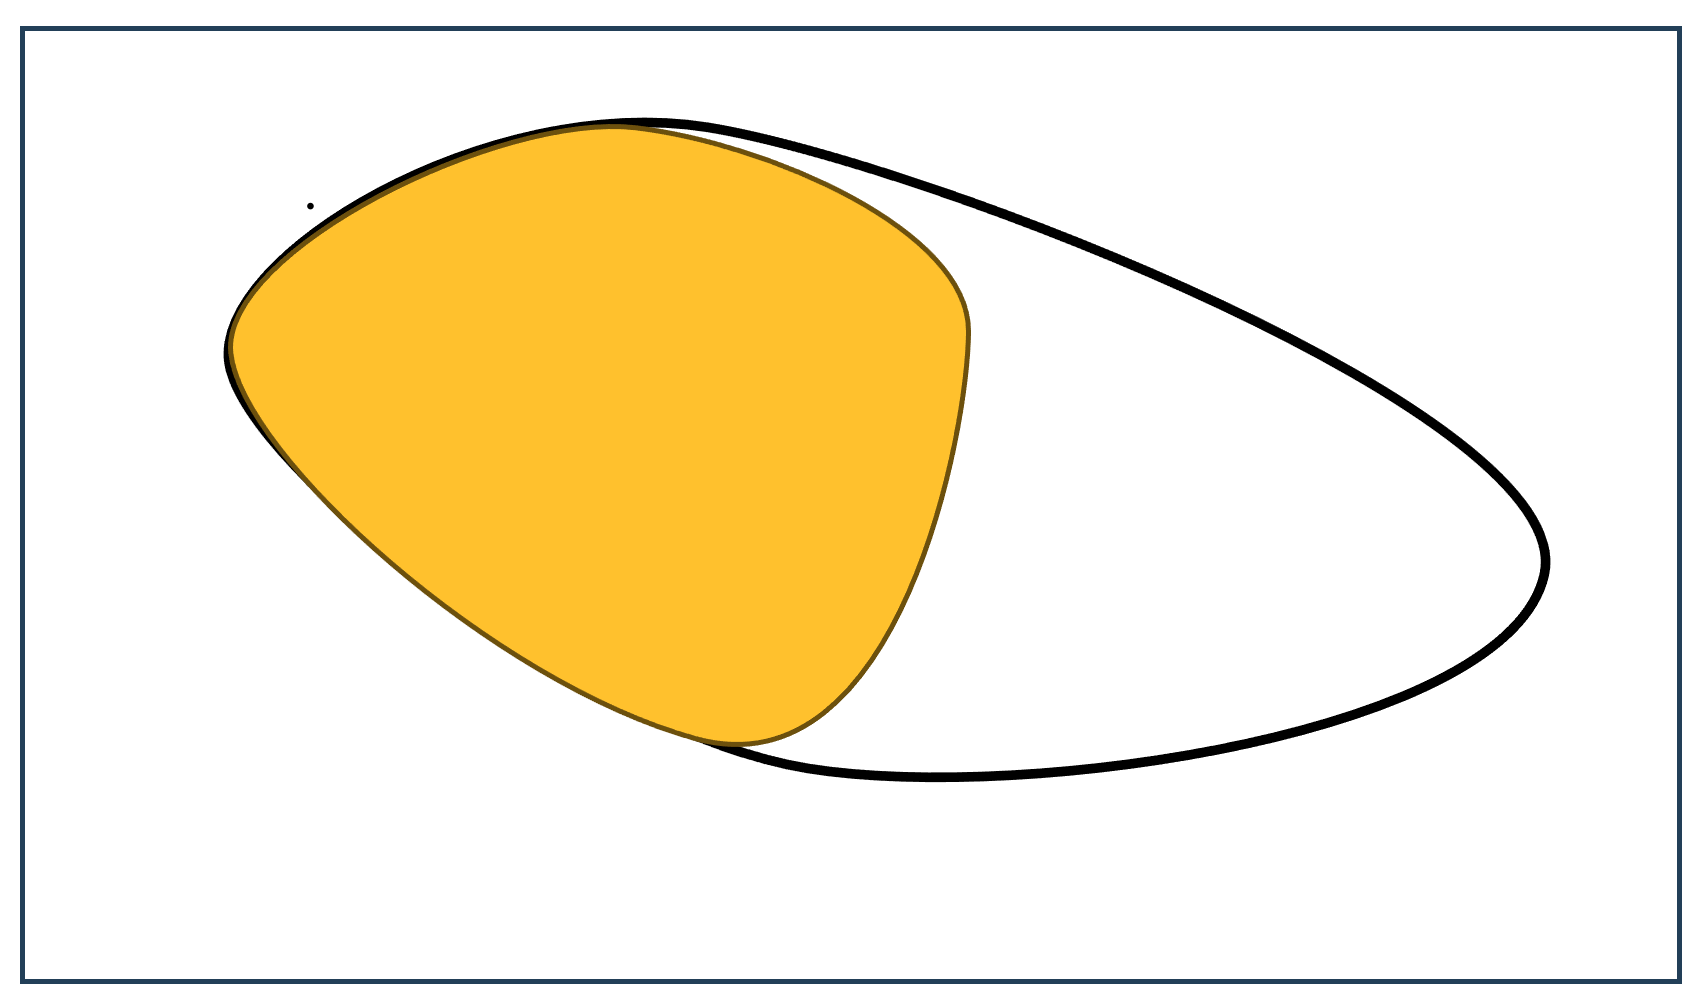
\includegraphics[scale=.2]{figs/VDPartition1.png} 
  	\end{center}
  	
	\vspace{4in}
	\end{frame}

\begin{frame}
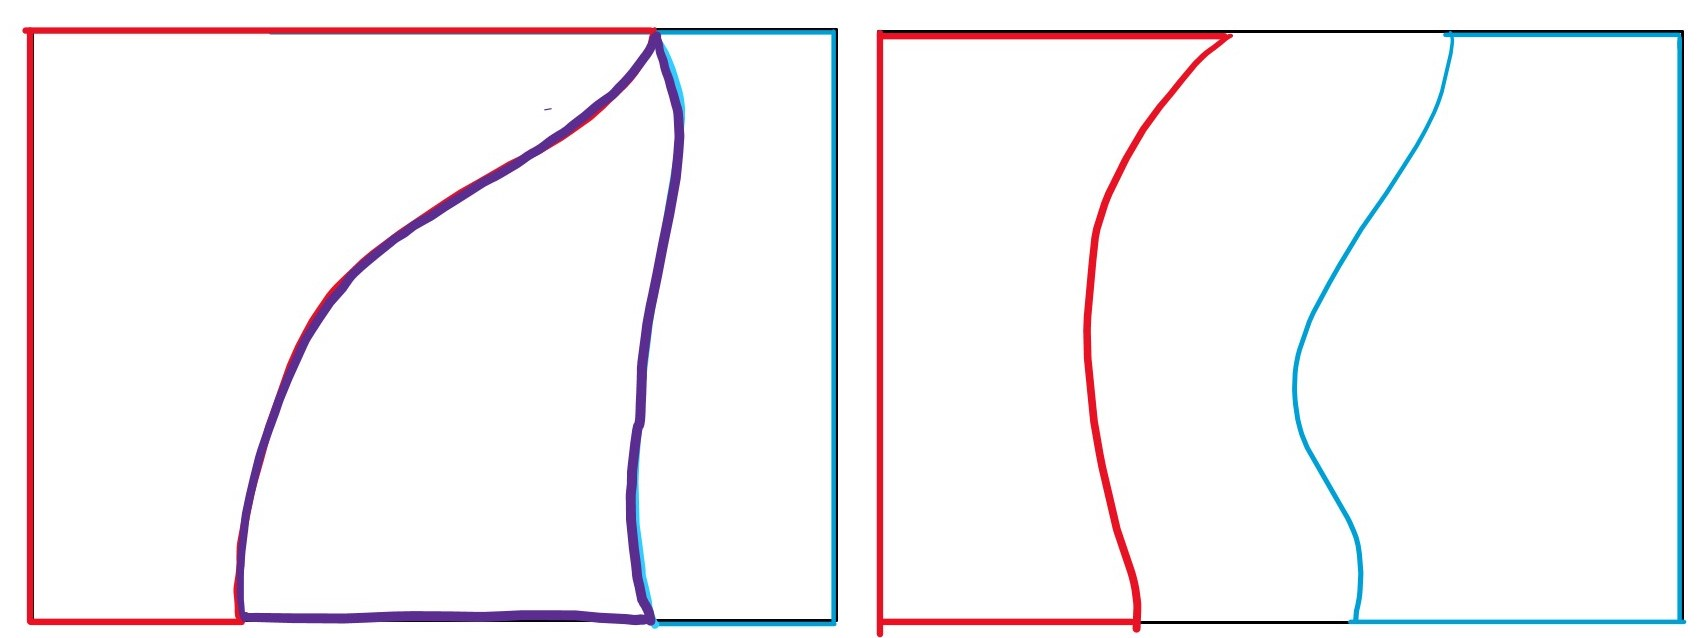
\includegraphics[scale=.42]{figs/BlankVD6.jpg} 
   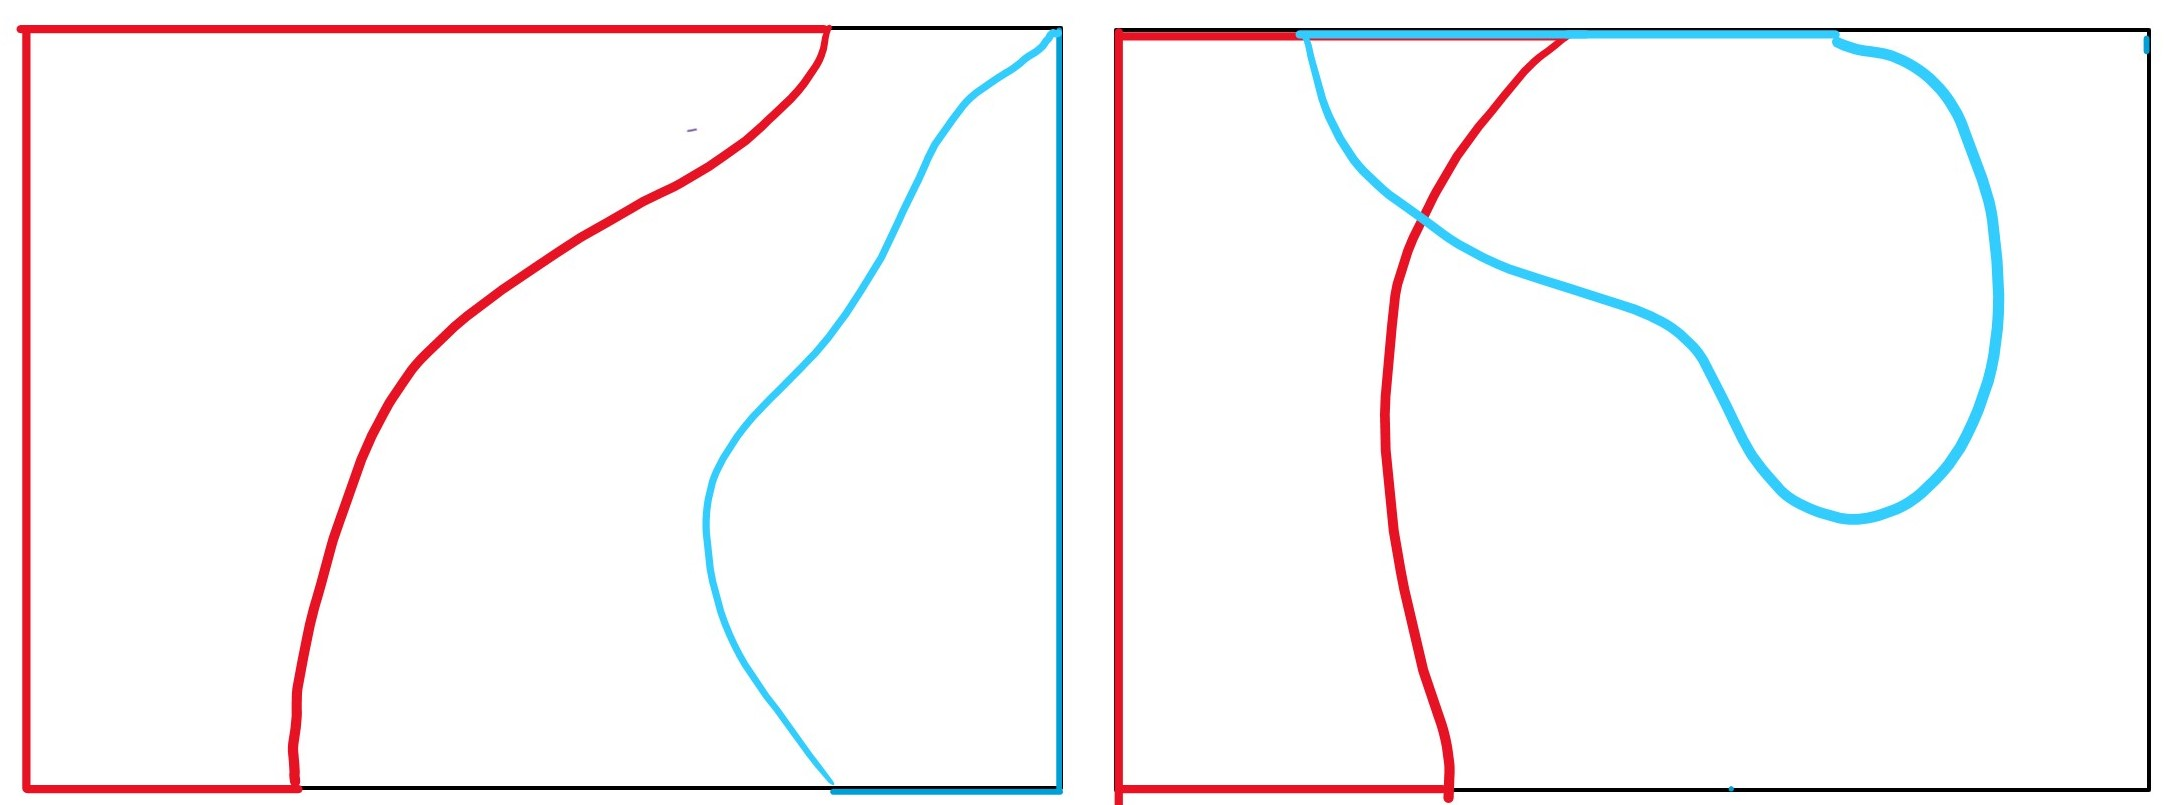
\includegraphics[scale=.32]{figs/BlankVD4.jpg} 
\end{frame}
\begin{frame}\frametitle{Example}
 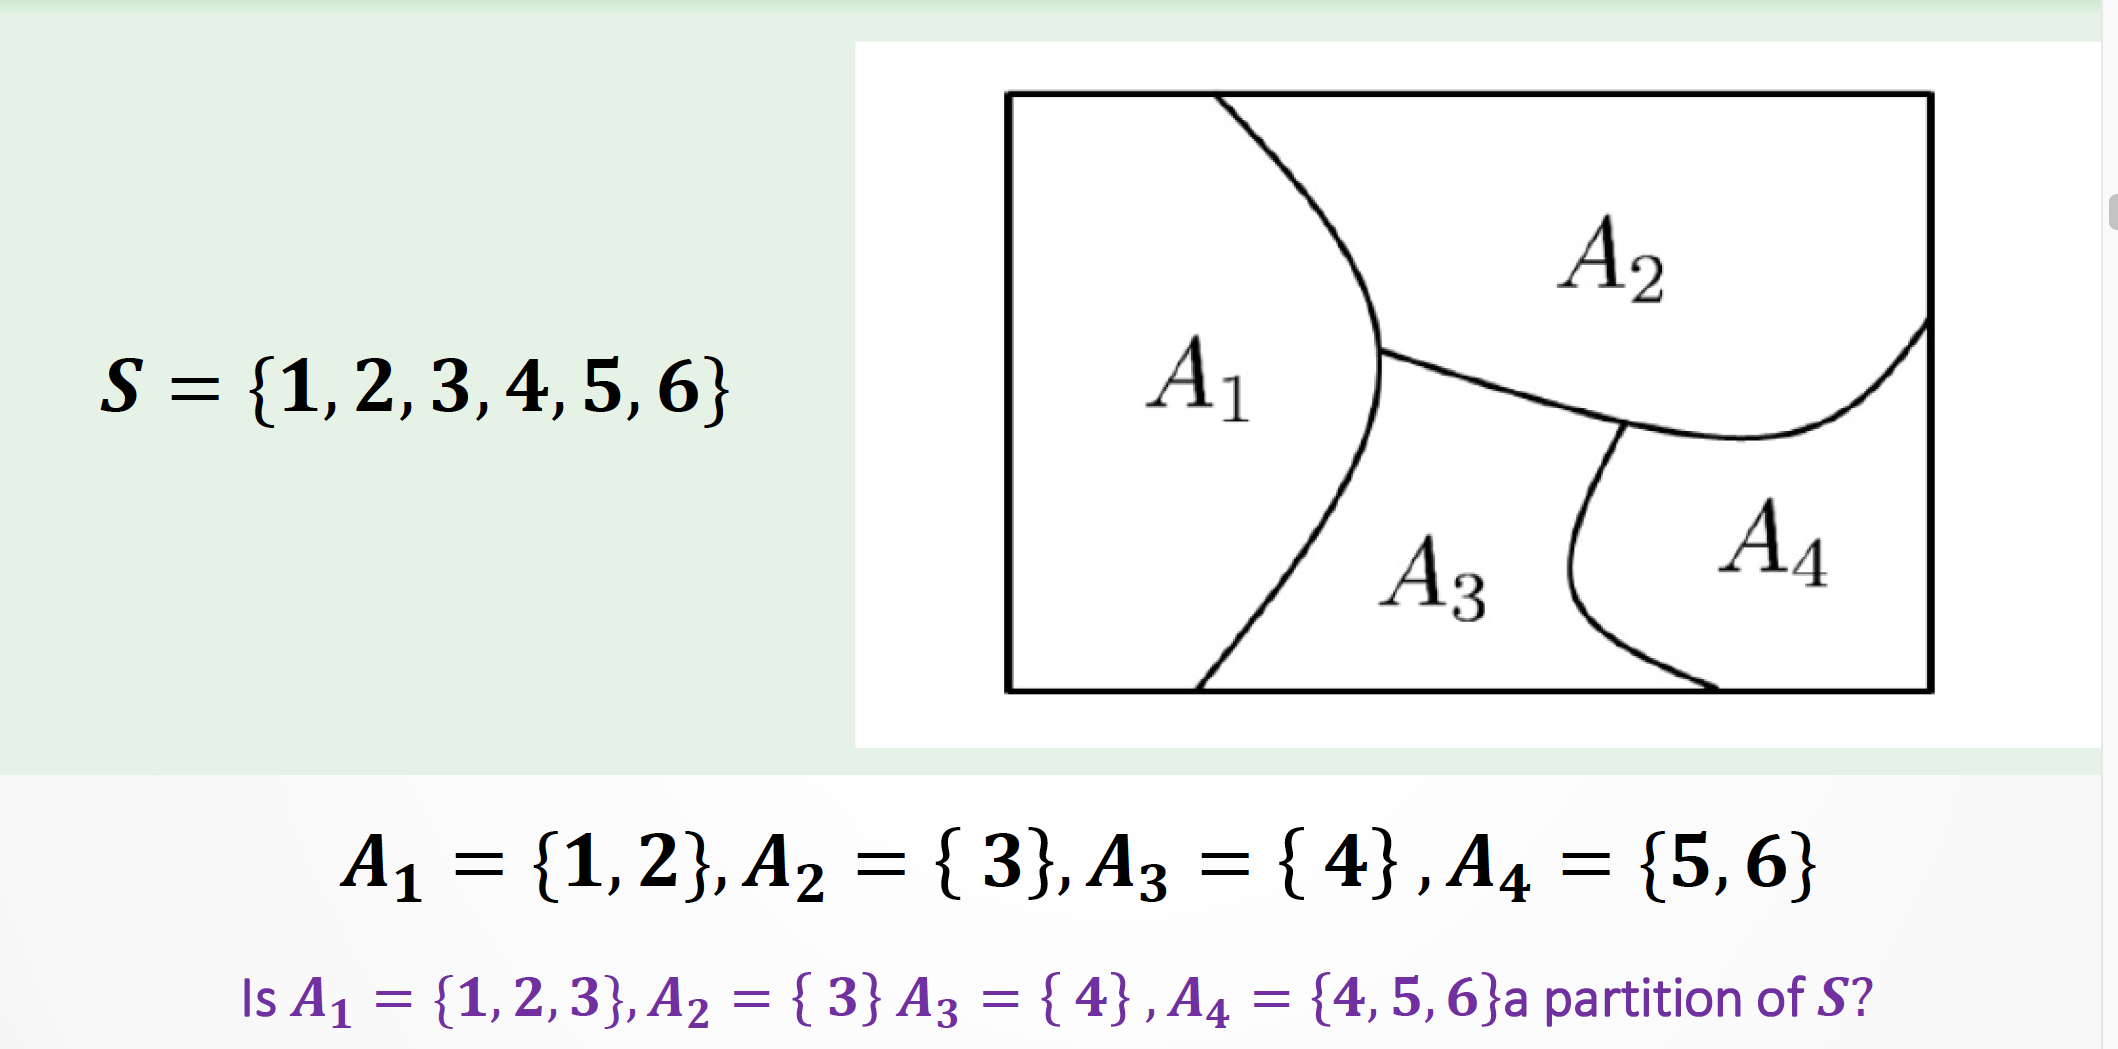
\includegraphics[scale=.34]{figs/VDPartition.png} 
\end{frame}

\begin{frame}\frametitle{Examples}

\end{frame}

\begin{frame}\frametitle{A Few Questions:}
Let $\Omega$ be the universal set and $\emptyset$ denotes the emptyset.  
\begin{itemize}
\item  $A \cup \emptyset=$
\item $A \cup \Not{A}=$
\item  $A \cap \emptyset=$
\item $A - \Not{A}=$
\item  $A \cap  \Not{A}=$
\item  $A \cup  \Omega=$
\item  $A \cap  \Omega=$
\item If  $A \subset B$ then $A\cap B=$
\item If  $A \subset B$ then $A\cup B=$
\end{itemize}


\end{frame}







\section{Real Numbers \& Intervals}
\TransitionFrame[antiquefuchsia]{\Large Real Numbers ($\R$) \& Intervals }

\begin{frame}\frametitle{Real Numbers, Intervals}
\qbx[4.5in]{amethyst!60}{
\begin{center}
For the definitions below, assume $\HLTW{a\in \R$, $b\in \R}$, and $\HLTW{a<b}$. 
\begin{enumerate}
\item[] \qBrd[2.5in]{blush!40}{\sqBullet{purple} $\HLTW{[a,b]}:=\{x\in \R : a\leq x\leq b \}$}
\item[] \qBrd[2.5in]{applegreen!40}{\sqBullet{olive}$\HLTW{(a,b]}:=\{x\in \R : a< x\leq b \}$}
\item[] \qBrd[2.5in]{brightpink!35}{\sqBullet{brightpink}$\HLTW{[a,b)}:=\{x\in \R : a\leq  x< b \}$}
\item[] \qBrd[2.5in]{babyblue!50}{ \sqBullet{capri}$\HLTW{(a,b)}:=\{x\in \R : a< x<b \}$}
\end{enumerate}
\end{center}
}
\vspace{3in}


\end{frame}


\begin{frame}\frametitle{Examples of Intervals}
 \vspace{.1in}
 
 \qBrd[4.55in]{burntsienna!40}{$\HLTW{[0,1]}:=\{x\in \R : 0\leq x\leq 1 \}$= {\tiny Set of all real numbers from 0 to 1, including the numbers 0 and 1. }}\\
 \vspace{.1in}
 
\qBrd[4.55in]{burlywood!40}{$\HLTW{(0,1)}:=\{x\in \R : 0< x< 1 \}$={\tiny Set of all real numbers between 0 to 1. It does not include the numbers 0, and 1. }}\\
 \vspace{.1in}
\qBrd[4.55in]{candypink!40}{$\HLTW{(0,\infty)}:=\{x\in \R : 0< x\}$={\tiny Set of all positive real numbers.  The interval {\bf does not include 0}}}\\
  \vspace{.1in}
 \qBrd[4.55in]{byzantium!40}{$\HLTW{[0,\infty)}:=\{x\in \R : 0< x \}$={\tiny Set of  all non-negative real numbers.  The interval {\bf does  include 0}}}
\vspace{2in}
\end{frame}

\begin{frame}\frametitle{Examples: Union \&  Intersection of Intervals}

\end{frame}



\section{The Notion of Cartesian Product}

\TransitionFrame[antiquefuchsia]{\Large The Notion of Cartesian Product  }
\vspace{-.1in}
\begin{frame}
	\frametitle{The Notion of `Tuple'}
	\qBrd[4.6in]{apricot!40}{\qBrd[.4in]{apricot}{\bf Tuple:} Let $k$ be an integer.  A {\bf $\HLTY{k}$-tuple} is the a the ordered sequence of values often written inside parenthesis while different elements are separated by comma. 
	}\\
	
	{\tiny 
	Example:
\begin{itemize}
\item  $(1.5, 2)$ is a {\bf 2-tuple}. 
\item  $(1.5, 2, 6, 2)$ is a {\bf 4-tuple}. 
\item $(H,T, H, H, H)$ is a {\bf 5-tuple}
\end{itemize}	
}
\vspace{2in}
	
	\end{frame}
	
	
	
	
	\begin{frame}\frametitle{Set Operation: Cartesian Product}
	\begin{center}
\qbx[4.3in]{teal!30}{\qBrd[2.1in]{olive!30}{\bf Cartesian Product of $A$ and $B$:}  Cartesian Product of $A$ and $B$,  denoted by  $\HLTY{A \times B}$ is the set of all ``two-tuple'' objects where the first element in the tuple is from the set A and the second element is taken from the set B. \\
}\\
\pause
\vspace{-.2in}
  \qbx[3in]{applegreen!50}{  
 $ A \times B=\{(x,y)\st x\in A, y\in B\}. $
  }
  	\end{center}
  	 {\tiny {\bf Comment:} In general $\HLTY{A\times B}$ is not same as $\HLTY{B\times A}$. However, $A\times A$ is denoted by $A^2$.  Note that $A$ is a set and not a number.   }
  	 
  	 
\qbx[4.5in]{teal!20}{\qBrd[2.3in]{olive!30}{Cartesian Product of Multiple Sets}
Let $A_1$, $A_2$, ..., $A_n$ are  non empty sets.  Then their Cartesian product is defined as  following:\\
$A_1\times A_2\times \ldots \times A_n= \left\{ (a_1, a_2, \ldots, a_n): a_i\in A_i \text{ for } i =1, \ldots n \right\}.$
}
	\vspace{4in}
	\end{frame}






\begin{frame}\frametitle{ A Few Standard Notation}
\vspace{-.08in}
\qbx[4.5in]{blue!40}{
\begin{itemize}
\item[]\qBrd[4.1in]{babyblue!40}{$\HLTW{\mathbb{Z}:\;\;}$ Set of all Integers.  i.e. $\mathbb{Z}=\HLTW{ \{0, -1, 1, -2, 2, -3, 3, \ldots \}}$.}\\
\vspace{-.2in}
\item[]  \qBrd[4.1in]{babyblue!70}{ $\HLTW{\mathbb{Z}_{+}:}$ Set of all non-negative Integers.  i.e. $\mathbb{Z}_{+}= \HLTW{\{ 1, 2, 3, \ldots \}}$.}
\end{itemize}	
}\\
\vspace{.1in}
	\qbx[4.5in]{amethyst!70}{
\begin{itemize}
\item[] \qBrd[2.6in]{blush!40}{$\HLTW{\R:\;\;}$ Set of all real numbers.  }
\item[] \qBrd[2.6in]{blush!60}{ $\HLTW{\R_+:}$ Set of all positive real numbers.  }
\end{itemize}	
}
\vspace{-.1in}

\pause
\qBrd[4.6in]{teal!40}{
\begin{itemize}
\item $\HLTW{\R^2}= \R\times \R=\HLTW{\{ \HLTY{(x_1,x_2)}: x_1\in \R, x_2\in \R\}}$
\item $\HLTW{\R^3}= \R\times \R \times \R=\HLTW{\{\HLTY{(x_1,x_2, x_3)}: x_1\in \R, x_2\in \R, x_3\in \R\}}$
\item  $\HLTW{\mathbb{Z}_{+}^2}=\mathbb{Z}_{+}\times \mathbb{Z}_{+}=\HLTW{\{\HLTY{(z_1,z_2)}: z_1\in\mathbb{Z}_{+}  , z_2\in \mathbb{Z}_{+}\}}$
\end{itemize}
}
\end{frame}






\TransitionFrame[tangerine]{\Large Discussion on Cardinality of Sets  }
\begin{frame}\frametitle{A Discussion on Cardinality of Various Sets}

\end{frame}
 
 
 
 \begin{frame}\frametitle{Finite Set}
 \qbx[4in]{babyblueeyes!80}{Examples: \\$ \{1, 2,3 , 4, 5 ,6\}$, \\
    $ \{HH, HT, TH, TT\}$}
\vspace{3in}

 \end{frame}






 \begin{frame}\frametitle{The Notion of Infinity ($\infty$)}
%\qbx[4.6in]{babyblueeyes!80}{\qBrd[0.8in]{babyblue!40}{
% Infinity ($\infty$):} Infinity,  denoted as $\infty$,  is a numeric concept that represent a  large    
%}
%\vspace{.5in}
 \end{frame}



 \begin{frame}\frametitle{Infinite Set: Countably Infinite Set}

\qbx[4in]{babyblueeyes!80}{Examples: $\HLTW{\mathbb{Z}_{+}:=\{1, 2, 3, \ldots, \}}$, $\HLTW{\mathbb{Z}_{+}^2}$}
\vspace{3in}
 

 \end{frame}
 
 
 
 
 \begin{frame}\frametitle{Infinite Set: Uncountable Set}
 \qbx[4in]{babyblueeyes!80}{ Examples:  $\HLTW{\R}$, $\HLTW{\R^2}$,   $\HLTW{\R_+}$  }
\vspace{3in}

 \end{frame}
 
 
 
 
 

\TransitionFrame[antiquefuchsia]{\Large Questions?  }
 
 
\end{document}
